\chapter{Bandwidth Aggregation Systems}\label{chap:network}

This chapter considers

% \begin{figure}
%   \centering
%   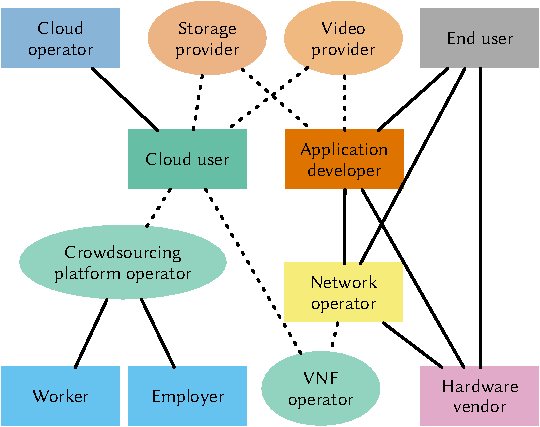
\includegraphics{network/figures/stakeholders}
%   \caption{Stakeholders investigated in the network scenarios.}
%   \label{fig:network:stakeholders}
% \end{figure}

Thus, a tradeoff between

Current best practices result in

The contribution of this chapter is threefold:
\begin{enumerate}
\item We provide an algorithm to infer metrics for the
\item We develop an analytical model in order to
\item We study the impact of
\end{enumerate}

The content of this chapter is taken from~\cite{info3-article-2016-3}.
Its remainder is structured as follows.
First, ...
Then, ...
Finally, we conclude this chapter with lessons learned in \refsec{sec:network:lessons_learned}.

\section{Background and System Description}\label{sec:aggregation:background}
In this section we describe different bandwidth aggregation approaches in praxis and present related work on the performance evaluation of bandwidth aggregation systems.
In addition, we describe our system model of bandwidth aggregation systems with offloading policy.

\subsection{Bandwidth Aggregation Approaches}\label{sec:aggregation:background:aggr}

The principle of sharing or offloading between multiple Internet access links is already widely used by commercial services as well as research work. WiFi-sharing communities like Fon\footnote{\url{http://www.fon.com}}, Karma\footnote{\url{https://yourkarma.com/}}, WeFi\footnote{\url{http://wefi.com/}}, and Boingo\footnote{\url{http://www.boingo.com/}} offer access to an alternative Internet link (WiFi instead of mobile), which provides a faster access bandwidth and reduces the load on stressed mobile networks. With respect to this so called ``WiFi offloading'', the research community investigated incentives and algorithms for access sharing \cite{mamatas2010incentives}, and ubiquitous WiFi access architectures for deployment in metropolitan areas \cite{sastry2007architecting, vidales2009metropolitan}. Moreover, \cite{lafuente2011flexible,donelson2012patent,seufert2013horst} describe systems for trust-based WiFi password sharing via an online social network (OSN) app. WiFi sharing is not a legal vacuum and a first exemplary overview on Swiss and French rights and obligations was given in \cite{camponovo2005wlan} but must be treated with caution due to international differences and interim law revisions.
The opposite concept to Wifi offloading, i.e., WiFi onloading, is presented in \cite{rossi20133gol}. The idea is to utilize different peaks in mobile and fixed networks to onload data to the mobile network to support applications on short time scales (e.g., prebuffering of videos, asymmetric data uploads).

%Bewifi
An access link sharing concept, which goes beyond pure offloading, is BeWifi, which was developed by Telefonica \cite{goma2013patent} and builds on previous works about backhaul capacity aggregation \cite{kandula2008fatvap,giustiniano2010fair}. BeWifi uses modified access points, which act as normal access points until their clients saturate more than 80\% of the backhaul capacity. Then, the access point will scan for close access points, which will provide additional bandwidth if their utilization is below 70\%. Backhaul capacity and utilization are announced by each access point via beacon frames. Instead of introducing a secondary WiFi radio, BeWifi uses time-division multiple access (TDMA) and the 802.11 network allocation vector (NAV) to connect to neighboring access points for bandwidth aggregation in a round robin fashion with a weighted proportional fairness schedule.

% The client-based solution requires driver modifications on the wireless clients.
% Each wireless client needs to feature a virtualized wireless card.
% This implies that for a commercial deployment the operating system and wireless driver of every WiFi client needs to be modified, which would produce a high amount of costs.
% %As one may realize, the cost of such an approach is absolutely prohibitive.
% The problem of the diversity of devices that need to be modified can be solved
% by deploying the aggregation scheme in the access points, which are usually provided by ISPs.
% However, current methods to perform aggregation with single-radio devices are not meant to be used in APs.
% Introducing a secondary WiFi radio in the APs could provide a technical solution, but it increases the cost of a device that is subsidized by the ISP, making the solution impracticable.

\reffig{fig:aggregation:background:aggr} shows a client-based and an access point solution for the bandwidth aggregation proposed in \cite{goma2013patent}.
The state of the art client-based system proposes to use a TDMA based access strategy for accessing selected access points in range in a round robin fashion, i.e., no concurrent data transmission via different frequencies is taking place.
The system utilizes inband signaling, a switching frequency of 100ms and requires less than 1.5ms for switching.
%The state of the art client-based aggregation schemes propose the use of TDMA to enable a single-radio client to connect to all the neighboring access points, as in \reffig{fig:aggregation:background:aggrclient} regardless of their frequency of operation. Over cycles of 100 ms the wireless client sequentially connects to all selected access points within range in a round robin fashion.
%The system utilizes inband signaling and requires less than 1.5 ms for switching.
Using the standard 802.11 power saving feature, a client is able to notify its absence to the access points it is connected to, so that they buffer packets directed to it.
A client performing aggregation appears to be sleeping in all access points but the one that is currently scheduled in the round robin cycle.
%No concurrent data transmission via different frequencies is taking place.
The access-point-based solution can be mapped to the client-based solution, if an access point acts as access point to its clients, and as a client to neighboring access points.
%single-radio AP that acts as an AP to its clients, and as a client to neighboring APs, and show that the problem can be mapped to the client-based solutions allowing the same optimization objectives

%acts as an AP and as a client of a neighboring AP
%the APs transmit on different channels
%The client-based solution is able to fully aggregate the available capacity of the
%backhaul links for a wider range of wireless channel capacities.
%their need for client modifications makes their deployment cost prohibitive.
%To unleash the potential of those solutions, the present invention provides and implements a system that can approach the benefits of client-based solutions requiring modifications only on the APs

\begin{figure*}[tb]
    \centering
    \begin{subfigure}[t]{0.5\textwidth}
        \centering
        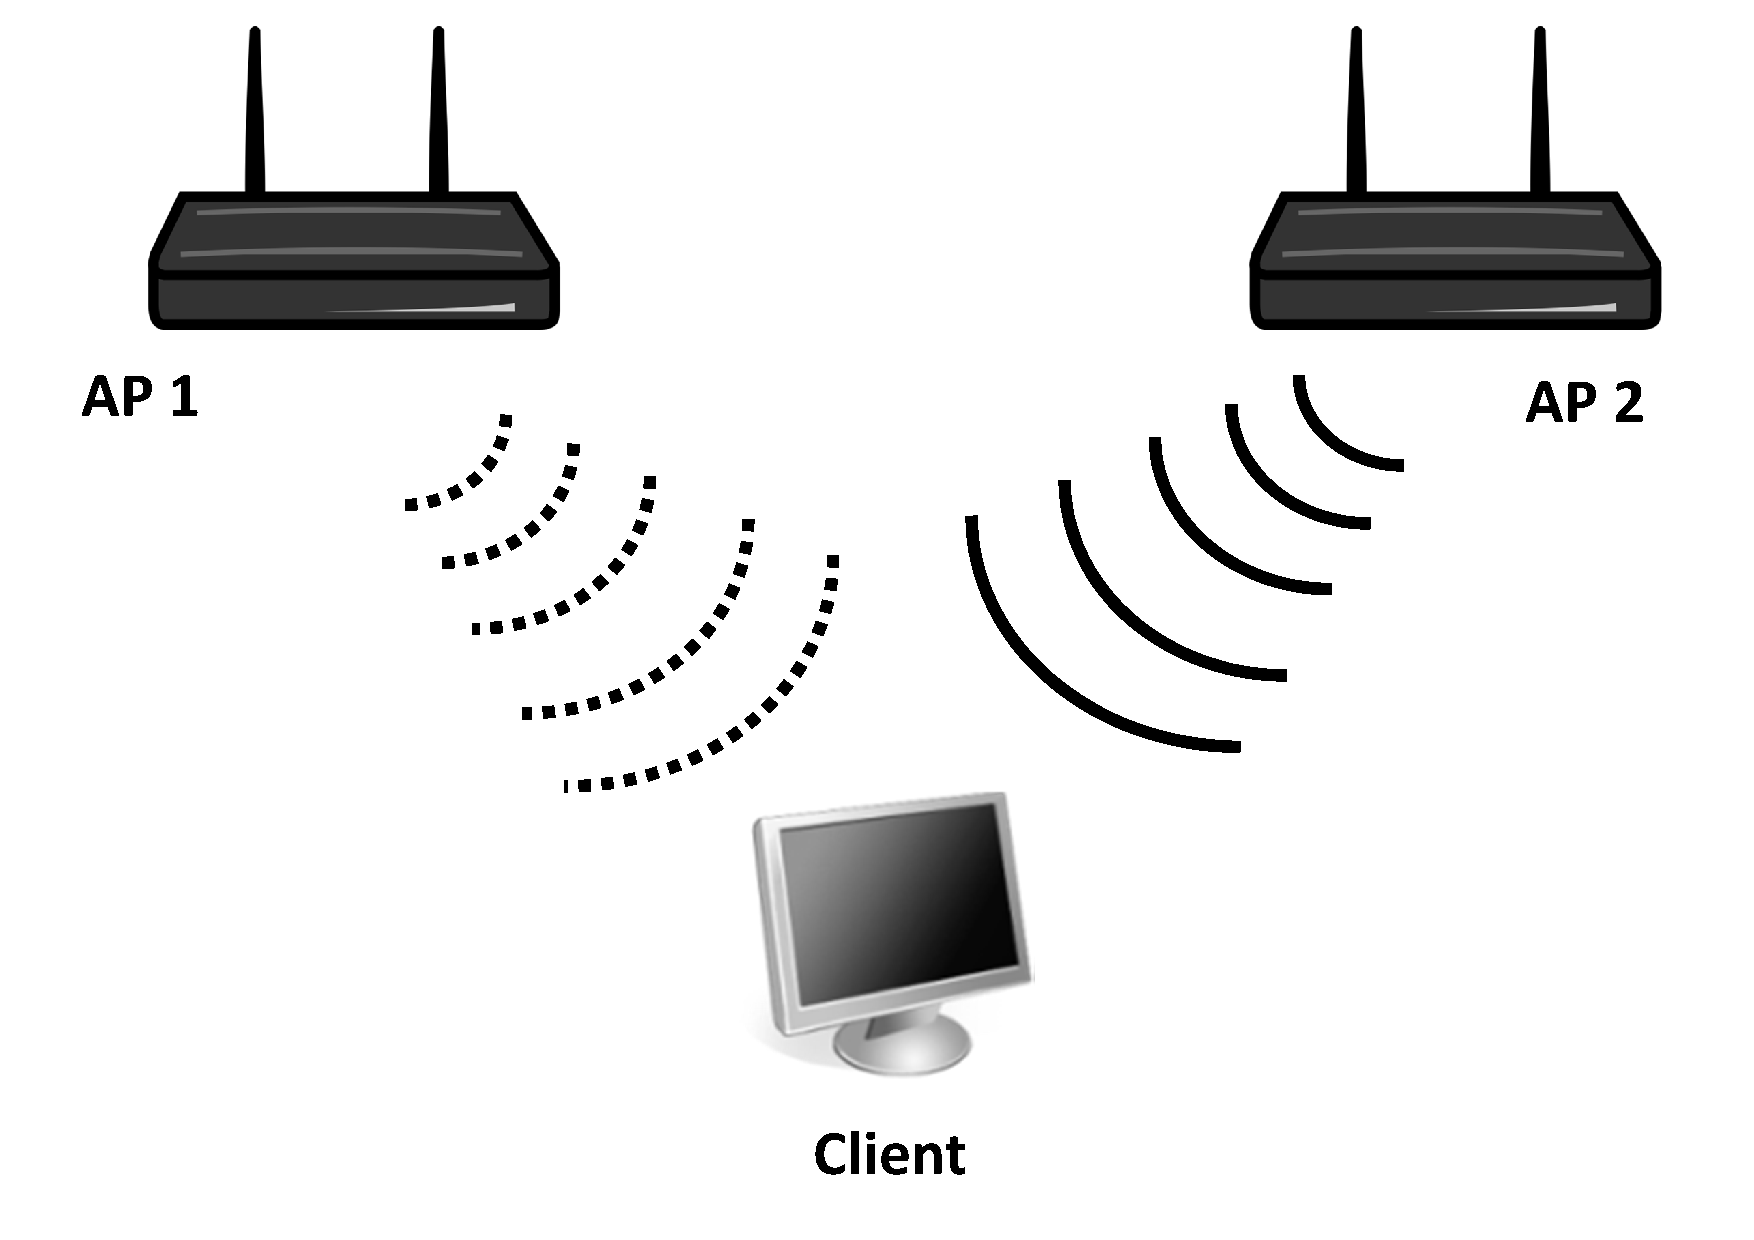
\includegraphics[width=.9\textwidth]{aggregation/background/figures/aggr_client_sw}
        \caption{Client-based}
				\label{fig:aggregation:background:aggrclient}
    \end{subfigure}%
    ~
    \begin{subfigure}[t]{0.5\textwidth}
        \centering
        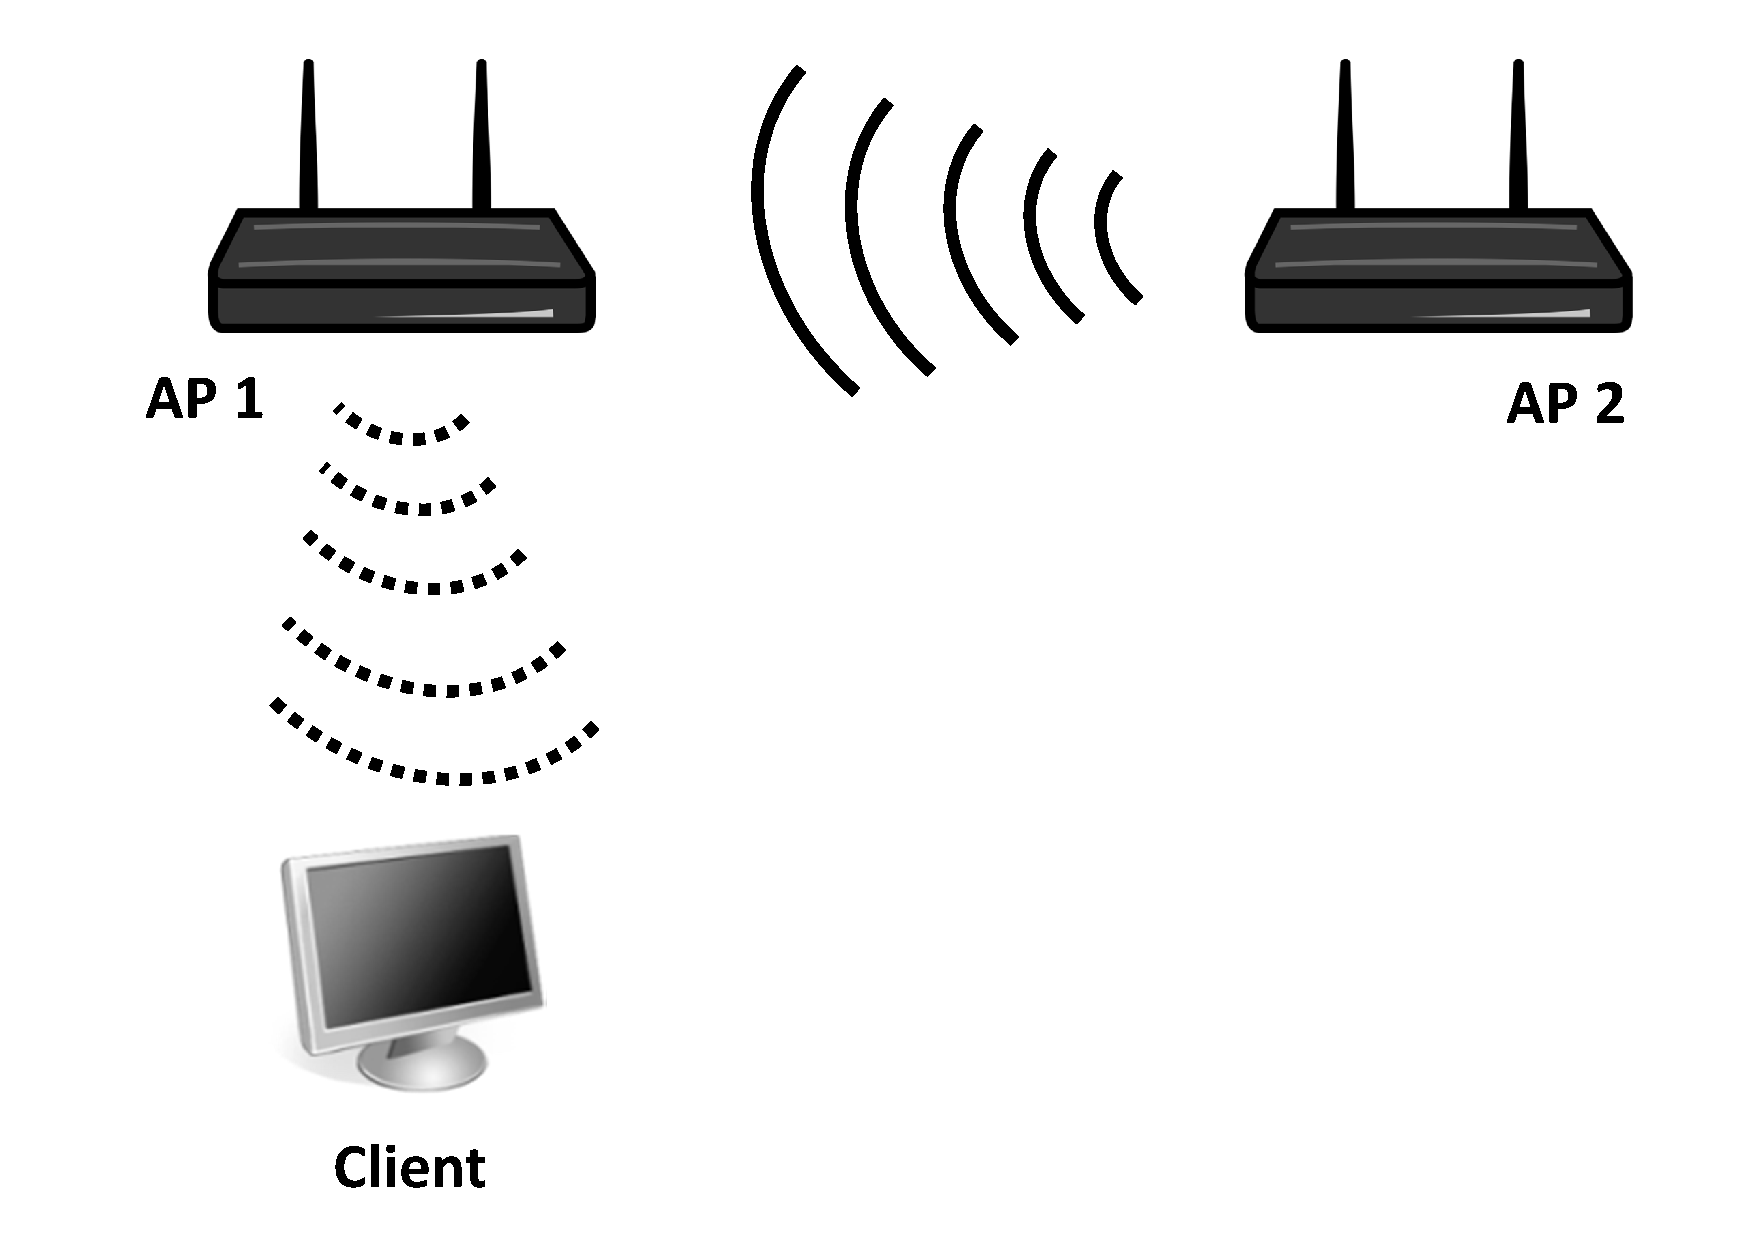
\includegraphics[width=.9\textwidth]{aggregation/background/figures/aggr_ap_sw}
        \caption{Access-point-based}
				\label{fig:aggregation:background:aggrap}
    \end{subfigure}
    \caption{Client-based and access-point-based solution for bandwidth aggregation.}
		\label{fig:aggregation:background:aggr}
\end{figure*}

From a technical perspective, bandwidth sharing and offloading are enabled by implementing handovers and/or multipath connections, which are well covered in research. \cite{gonzalez2013radio,paasch2012exploring,chen2013energy} show the feasibility of multipath TCP for handovers between mobile and WiFi networks in the current Internet and \cite{khadraoui2014survey} describes available features for mobile traffic offloading. Futhermore, \cite{gladisch2014survey} gives an overview on approaches that enable mobility and multihoming.
%In \cite{shifrin2010c3} a collaborative token bucket algorithm, which implements an effective distribution of the transmission rates is analyzed to evaluate the performance of wireless ad-hoc and mesh networks.

\subsection{Perfomance Models for Bandwidth Aggregation Systems}\label{sec:aggregation:background:models}

Theoretically, bandwidth sharing between WiFi access points can be considered as load sharing among systems.
Generally load sharing systems can be classified in partitioning, partial sharing and complete sharing systems.
Partitioning systems work completely independent from each other.
Each system has its own queue and buffer space and processes only requests arriving at its queue.
Complete sharing systems have a shared queue and buffer space. When processed, a request in the shared queue is assigned to the system which is currently least loaded.

Partial sharing systems have their own queues, but may offload requests to other systems if they are overloaded, or process requests from other overloaded systems.
Different partial sharing or complete sharing models have been investigated in literature.
In \cite{trangia1993trunk} the bandwidth usage by different services in a broadband system in complete sharing and partial sharing mode with trunk reservation is investigated.
Multidimensional Markov chains are used in \cite{chen2002performance,zhang2006dynamic,ke2010performance} to evaluate the performance of cellular network systems with different service categories.
The blocking probability of a complete sharing system has been approximated in \cite{kaufman1992blocking}.
This approximation is used in \cite{fodor2007bounding} to evaluate the performance of mobile networks with code division multiplexing supporting elastic services.
However, none of the models can be used to seamlessly evaluate the performance of systems between partitioning and complete sharing.

Thus, we develop a model based on a two dimensional Markov chain with thresholds to study the transition of blocking probabilities of partitioned, partial sharing, and complete sharing systems.
%The Markov model is limited to two access links only.
This limits its applicability, since the number of average WiFi access points visible to clients is much higher in densely-populated areas.
In densely-populated areas bandwidth of a high number of WiFi access points is aggregated. In this case an assessment with the Markov model  is not possible, since it is limited to two access links. An extension of the Markov model to $m$ dimensions would require solving an equation system with $n^m$ equations, which is computationally too complex.
Therefore, we extend the model to be applicable to multiple access links by utilizing a fixed point approximation.

The fixed point approximation is used to reduce the m-dimensional Markov chain to one dimension similar to \cite{trangia1992polling, staehle2002approximation}, where the approach is used for analytic models for polling systems and the interference distribution in UMTS networks, respectively.
The underlying Markov chain highly differs from existing fix-point approaches, since it considers support and offloading thresholds.
To the best of our knowledge this is also the first work that considers an inner and an outer composite system to apply the fixed point analysis in heterogeneous load conditions.

%multipath transmissions
%Multipath transmissions?
%von hossi:
% Survey on Mobility and Multihoming in Future Internet: http://link.springer.com/article/10.1007/s11277-012-0898-6#page-1
% A Survey of Available Features for Mobile Traffic Offload: http://ieeexplore.ieee.org/stamp/stamp.jsp?tp=&arnumber=6843152
% Exploring Mobile/WiFi Handover with Multipath TCP: http://inl.info.ucl.ac.be/system/files/cell06-paasch.pdf
% An Energy-aware Multipath-TCP-based Content Delivery Scheme in Heterogeneous Wireless Networks: http://www.eeng.dcu.ie/~munteang/papers/2013_WCNC_SC.pdf
% Radio access considerations for data offloading with multipath TCP in cellular/WiFi networks: http://ieeexplore.ieee.org/xpl/freeabs_all.jsp?arnumber=6496709&abstractAccess=no&userType=inst

\subsection{System Model}


For simplicity and mathematical tractability we make assumptions on the link capacities and the service rates of bandwidth fractions. This allows analytic performance evaluation of bandwidth aggregation systems with offloading policy and understanding its characteristics.


%\newtheorem{amp4}[amp1]{Assumption}\label{amp:traffic}
%\begin{amp4}
%	The arrivals of traffic bursts follow a Poisson process.
%\end{amp4}

%There are different effects in real systems, which are not considered in the model.

\newtheorem{amp1}{Assumption}\label{amp:switching}
\begin{amp1}
	The switching time to another access link is zero.
\end{amp1}
In practice, TDMA is used to aggregate the bandwidth of two access points operating on different channels.
During the time in which the client is switching frequencies, it cannot send or transmit data. This time is called switching time and for state of the art systems it is 1.5ms \cite{goma2013patent}.
This switching time slightly decreases the effective throughput of the system.
Signaling among the cooperating access points is necessary to report the current load and the offloading state.
The messages exchanged produce a signaling overhead, which can limit the performance of the system.
In practice APs announce their backhaul link capacity through Beacon frames, as well as their available-for-aggregation throughput, i.e. the part of their capacity that is not utilized by their clients \cite{goma2013patent}.
However, in \cite{goma2013patent} the aggregate throughput remains almost constant across the different experiments, indicating that the overhead of switching and signaling is fixed and only slightly impacts the overall throughput.
\newtheorem{amp2}[amp1]{Assumption}\label{amp:aggrlimit}
\begin{amp2}
	The wireless channels are clean.
\end{amp2}
Interference can limit the capacity of the wireless links.
The effect of the channel quality on the aggregation capacity is evaluated in \cite{goma2013patent}.
To account for a bad channel quality in our model, the link capacity can be reduced accordingly.

\newtheorem{amp3}[amp1]{Assumption}\label{amp:servicetimes}
\begin{amp3}
	The service time of bandwidth fractions follows a negative exponential distribution.
\end{amp3}
%In practice, the link throughput has low variations which makes the service time of traffic bursts more deterministic.
%As shown in \cite{burger2016phycom} for two cooperating systems, the Markov model also provides good approximations for the received bandwidth and blocking probability for deterministic and highly variant service time distributions.

%%We think that these effects are marginal and negligible on high loads.
%As these effects have only marginal impact on the system performance, they are neglected in the model.
%By making the assumptions, we can evaluate the performance of bandwidth aggregation systems with offloading policies analytically and understand its characteristics.

%develop a solution that can enable the desired functionality simply through software AP modifications and without any client support

%a single-radio AP that acts as an AP to its clients, and as a client to neighboring APs, and show that the problem can be mapped to the client-based solutions allowing the same optimization objectives,

%More importantly, if the two metrics are add up, the aggregate throughput remains almost constant across the different experiments, indicating that the overhead of switching from AP to client is fixed and only impacts overall aggregate throughput by 3.2 Mbps

%This value is actually w11switching=0:86 xW11-No-Switching. This shows the impact of the channel switching overhead.

%potential of those solutions, the present invention provides and implements a system that can approach the benefits of client-based solutions requiring modifications only on the APs.

%\subsection{Model Limitations}
%
%The model has limitations. A critical part of the model are the negative exponential service times, which may in reality be more deterministic, since the link throughput has low variations.
%However, as will be shown in section \ref{sec:simgeneral} the model also provides good approximations for the received bandwidth and blocking probability for different service time distributions.
%There are different effects in real systems, which are not considered in the model.
%For example signaling among the cooperating access points is necessary to report the current load and the offloading state.
%The messages exchanged produce a signaling overhead which can limit the performance of the system.

%To use Markov chain model analysis, we assume in the following that the processes
We model the load on $m\geq 2$ access links as depicted in Figure~\ref{fig:aggr:sysmodel}. The throughput of each Internet connection is limited by a bottleneck (either on application side, on server side, or in the core Internet), such that single connections will utilize a certain share of the access link bandwidth. Therefore, the available capacity of a link $c$ is divided into a number $n$ of small atomic bandwidth fractions of equal size. This means, $c = n\cdot \xi$ with a global constant $\xi$ denoting the granularity of bandwidth allocation. Thus, different capacities $c_i$ are modeled by assigning different $n_i$ to the links.

\begin{figure}[tb]
	\centering
 	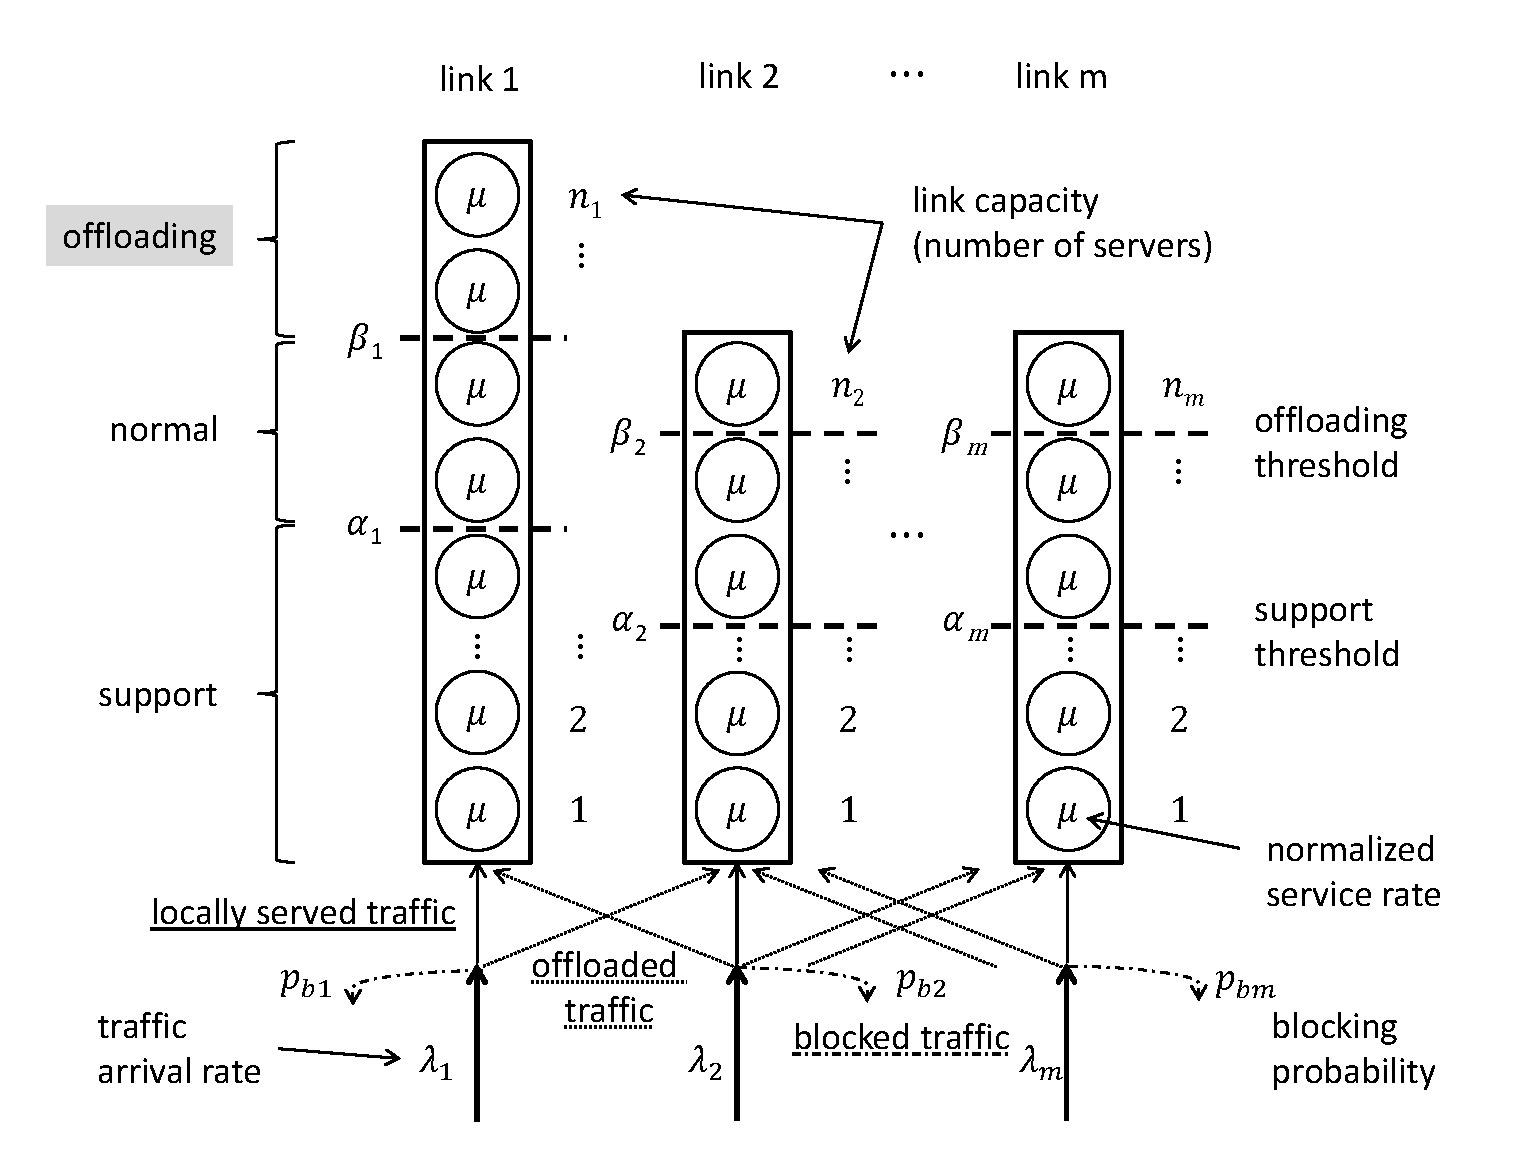
\includegraphics[width=0.9\textwidth]{aggregation/performance_model/figures/model_m}
  	\caption{System model.}
  	\label{fig:aggr:sysmodel}
\end{figure}

%In our scenario, we look at loaded access links on a short time scale. The throughput of each Internet connection is limited by a bottleneck (either on application side, on server side, or in the core Internet), such that the capacity of an access link cannot be fully utilized by a single connection. This means, each Internet connection will utilize a certain share of the access link bandwidth. The available capacity of a link $c$ is divided into a number $n$ of small atomic bandwidth fractions of equal size. This means, $c = n\cdot \xi$ with $\xi$ resembling the granularity of bandwidth allocation. For example, a $c=10\ \text{Mbps}$ link can be modeled as $n=20$ bandwidth fractions of $\xi=500\ \text{kbps}$ each, or also as $n=100$ bandwidth fractions of $\xi=100\ \text{kbps}$ each. For the remainder of this paper, we will consider $\xi$ as a global constant in the given scenario and model different capacities $c_i$ by assigning different $n_i$ to the links.
%short time frame load on links can be as stationary small variations poisson process

We consider the system in a short time frame, where the system load can be considered stationary.
Each access link is modeled as a multi-server blocking system, in which each server represents an available bandwidth fraction of the link.
Its utilization variations are modeled as a stationary process of singular and independent arrivals of traffic bursts, i.e., bandwidth fraction requests. This allows modeling an access link as M/M/n loss system \cite{kleinrock1975queuing}. We define $X$ as the random variable of the number of occupied bandwidth fractions on each backhaul link. It is modeled by a birth-death-process, in which bandwidth fractions are requested with Poisson arrivals at rate $\lambda$ and occupied for an negative-exponentially distributed service time with globally normalized rate $\mu=1$. Consequently, the load on each link is given by $\rho=\frac{\lambda}{n\cdot \mu}=\frac{\lambda}{n}$. The probability that $k$ bandwidth fractions are occupied in the considered M/M/n queue is $x(k)=P(X=k)$.

In the BeWifi approach (cf.~\refsec{sec:aggregation:background:aggr}), two thresholds are used, which define the bandwidth aggregation/offloading policy. The support threshold $\alpha$ indicates up to which percentage of utilization (i.e., number of own occupied bandwidth fractions) the system will offer bandwidth fractions to other systems. Furthermore, the offloading threshold $\beta$ with $\alpha\leq\beta$ sets the percentage of utilization above which the system will try to use bandwidth of other systems. According to these thresholds, a system can be in one of the following three macro states:

\begin{enumerate}
	\item \textit{support} ($0 \leq X < \lfloor\alpha\cdot n\rfloor$):\\ low utilization and offering bandwidth \, ,
	\item \textit{normal} ($\lfloor\alpha\cdot n\rfloor \leq X < \lfloor\beta\cdot n\rfloor$):\\ normal operation \, ,
	\item \textit{offloading} ($\lfloor\beta\cdot n\rfloor \leq X \leq n$):\\ high utilization and offloading to other systems \, .
\end{enumerate}

By applying the offloading policies, different Internet access links will collaborate and share traffic. More details on the investigated scenarios are presented in the following section.

Two bandwidth aggregation systems, i.e., systems offloading between $m$ access links, will be analyzed. First, we consider a bandwidth aggregation system with equal load on each access link. Moreover, a system in which one access link has a different load than the other $m-1$ links is modeled. As reference system we considered partitioned systems without offloading.% and a complete sharing system.

\subsection{Analysis of Reference Systems}

We compare the bandwidth aggregation gain of multiple collaborating Internet access links to a partitioned system without offloading. %, although it has to be noted that in many practical cases complete sharing is physically not possible.
The received bandwidth of each access link $E[X_i]$ and the blocking probability $p_{b_i}$ of each system $i$ are evaluated. The blocking probability gives the probability that the link is fully utilized and a bandwidth request of an application cannot be entirely satisfied. In practice, if TCP is used on the access link, the Internet connections throttle themselves and share the link equally. Depending on the used application and its characteristics, the application performance can then suffer, which can result in user dissatisfaction.

\subsubsection{Partitioned and Complete Sharing Systems}

For completely partitioned systems, i.e., $m$ different M/M/$n_i$ loss systems with arrival rates $\lambda_i,\ i\in\{1,\ldots, m\}$, the received bandwidths $E_0[X_i]$ can be computed individually for each access link by Little's Theorem as
\begin{equation}
E_0[X_i] = \frac{\lambda_i}{\mu}\cdot(1-p_{b_i}),% = \lambda_i\cdot(1-p_{b_i})\ ,
\end{equation}
in which we use the rate of accepted arrivals $\lambda_i\cdot(1-p_{b_i})$ and the globally normalized service rate $\mu=1$.

The blocking probability of partitioned systems $p_{b_i}$ follows from the Erlang-B formula \cite{kleinrock1975queuing}
\begin{equation}
p_{b_i} = \frac{\frac{(\frac{\lambda_i}{\mu})^{n_i}}{n_i!}}{\sum_{k=0}^{n_i}\frac{(\frac{\lambda_i}{\mu})^{k}}{k!}}\ .
\end{equation}

The performance $E_s[X]$ of a complete sharing system, i.e., a single M/M/n loss system with $n=\sum_{i=1}^m n_i$ servers and an arrival rate of $\lambda=\sum{i=1}^m \lambda_i$, can be computed by the same formulae.

\subsubsection{Approximations and Performance Metrics}

An approximation $\tilde{p}_b$ of the blocking probability $p_b$ can be calculated by the joint probability of a single system being fully occupied, while a separate single system is above the support threshold $\alpha$, i.e. could not help. If $X_1$ and $X_2$ are random variables for the number of jobs in system 1 and system 2, the joint probability is

\begin{equation}
\tilde{p}_b = P(X_1=n_1,X_2\geq \alpha\cdot n_2) = P(X_1=n_1)\cdot P(X_2\geq \alpha\cdot n_2)\ .
\end{equation}

Moreover, we analyze the mean total number of occupied bandwidth fractions $E[X]$% as well as the mean number of occupied bandwidth fractions $E[X_i]$ of each system
, which corresponds to the mean of total aggregated bandwidth. Following the same argumentation as above, $E[X]$ can be computed by Little's Theorem as
\begin{equation}
E[X] = \frac{\lambda_1+\lambda_2}{\mu}\cdot (1-p_b) = \frac{\lambda_1}{\mu}\cdot (1-p_{b_1})+\frac{\lambda_2}{\mu}\cdot(1-p_{b_2})\ .
\end{equation}

Finally, we take a look at the received bandwidth at each access link $E[X_{A_i}]$. Thereby, $X_{A_i}$ is a random variable for the number of bandwidth fractions (in all systems), which are occupied by arrivals from system $i$. It is obvious that $E[X_{A_i}] = E[X_i]
 = E_0[X_i]$ for the partitioned system. In case of offloading, $E[X_{A_i}]$ can be calculated from the mean total number of occupied bandwidth fractions by taking into account the share of accepted requests from each system.
\begin{equation}\label{equ:gain}
E[X_{A_i}] = \frac{\lambda_i(1-p_{b_i})}{\lambda_1(1-p_{b_1})+\lambda_2(1-p_{b_2})}\cdot E[X] = \frac{\lambda_i}{\mu}\cdot (1-p_{b_i})
\end{equation}

Nevertheless, it is the goal of bandwidth aggregation to cooperate in order to use spare capacity on access links to increase the received bandwidth where needed. Therefore, we can quantify the percentage of bandwidth gain for each system as
\begin{equation}
\omega_i = \frac{E[X_{A_i}]-E_0[X_i]}{E_0[X_i]}\ .
\end{equation}

\subsection{Simulation Description}
A discrete-event based simulation using arrival and departure events is implemented to validate the analytic model and to assess the system performance in more general cases. Each of the $m$ systems has a Poisson arrival process with rate according to its load. The service time of bandwidth fractions is exponentially distributed with mean 1. Offloading decisions are made according to the the number of occupied bandwidth fractions in the systems with respect to the support and offloading threshold. Therefore, the simulation state holds the requests being processed and the number of occupied bandwidth fractions for each system.

% \section{Inferring Signalling Frequency and Power Consumption from Network Traces}\label{sec:network:network_traces}
All participating stakeholders, i.e. network operators, hardware vendors, and application developers, need to assess the impact of potential changes of parts of the mobile network, e.g. change of network parameters, introduction of new hardware or modification of applications, on their considered \glspl{KPI} without rolling out changes to the production network.
To this end, we propose specific metrics in order to quantify the impact of changes on the network on the considered \gls{KPI}.
We introduce an algorithm to infer metrics from application traffic measurements, network parameters and power and signalling configurations.
In \refsec{sec:network:network_traces:performance_evaluation} we present the algorithm and methods to describe the relevant metrics.
Then, in \refsec{sec:network:network_traces:numerical_results}, we use the proposed methodology to evaluate the impact of various network configurations on four popular applications.

\subsection{Comparison of Traditional and Virtualised Approach}\label{sec:cloud:virtualized_network_functions:performance_evaluation}

We implement the models introduced in \refsec{sec:cloud:virtualized_network_functions:model} using a \gls{DES} with the SimPy\footnote{\url{https://simpy.readthedocs.org/}, \accessed} package as foundation.
The implementation\footnote{\url{https://github.com/fmetzger/ggsn-simulation/}, \accessed} as well as the considered scenarios\footnote{\url{https://github.com/cschwartz/ggsn-simulation-studies/}, \accessed} are also publicly available as a reference.
To be in line with the measurement data we consider a simulation time for all simulation scenarios of 7 days, with a transient phase of 60 minutes.
Ten replications of each scenario were performed.
All error bars given in this section show the \SIrange{5}{95}{\percent} quantiles of all replications.

We use the measurements introduced in \refsec{sec:cloud:virtualized_network_functions:measurement_data} in order to dimension a traditional \gls{GGSN} as a baseline for all further studies.
Based on these results, we first examine the effects of network function virtualisation by scaling \emph{out} instead of up through a virtual \gls{GGSN} model.
Finally, we arrive at a more realistic version of the virtual \gls{GGSN} by taking the start-up and shut-down times into account.

\subsubsection*{Traditional \headershortacr{GGSN}}\label{sec:cloud:virtualized_network_functions:performance_evaluation:traditional_ggsn}

Employing the inter-arrival times and duration of tunnels, we first study the traditional \gls{GGSN} model introduced previously.
Whilst our measurements provide us with information on the frequency of new tunnels and the duration they remain active, we have no reliable information on the number of active tunnels the \gls{GGSN} can support.
Thus, in a first step, we dimension the \gls{GGSN} in such a way that a suitable blocking probability \(\blockingprobability\) can be achieved.

In order to obtain a baseline dimensioning, we perform a simulation study, considering the impact of an increasing offered load on the blocking probability.
We observe that as the number of supported parallel tunnels increases, the blocking probability decreases.
For the normalized inter-arrival no blocking is occurring if we allow for more than \(5000\) parallel tunnels.
Thus, we consider the range of \(4000\) to \(5000\) parallel tunnels to be of special interest for the remainder of the study.

\subsubsection*{Virtual \headershortacr{GGSN}}\label{sec:cloud:virtualized_network_functions:performance_evaluation:virtual_ggsn}

To study the feasibility of the virtual \gls{GGSN} approach discussed in \refsec{sec:cloud:virtualized_network_functions:model}, we compare the performance metrics of the virtual \gls{GGSN} with that of a traditional \gls{GGSN}.
To this end, the virtual \gls{GGSN} is simulated in varying configurations.
The number of servers and supported tunnels per server is chosen in such a way that the results can be compared with those obtained from our study of the traditional \gls{GGSN}.
Due to simulation time constraints, only a representative subset of scenarios is simulated.

In the virtual \gls{GGSN} model, servers are activated and deactivated on demand, while in the traditional \gls{GGSN} model, the single server is always on.
For this investigation a conservative start-up and shut-down time \(d\) of \SI{300}{\second} is chosen.
Generally, deactivating server instances reduces energy consumption, frees up inactive servers for other use, or reduces cost to be paid to a cloud operator.
For this reason, the number of active servers \(I\) is a relevant performance metric in the virtual \gls{GGSN} model.

\begin{table}\caption{Manipulation check for the experimental factors based on one-way ANOVA.}
\centering
\label{tab:cloud:virtualized_network_functions:performance_evaluation:virtual_ggsn:manipulation}
\tabcolsep=0.11cm
\begin{tabular}{lccccc}
\toprule
& \(F(2,1275)\) & \(\eta^2_p\) & \(p\) & Cohen's & Cohen's\\
&  & & & \(f^2\) & \(\hat{\omega}^2\) \\
\midrule
\emph{blocking probability} \(\blockingprobability\)  & & & & &\\
maxTunnels \(n\)&  15601.53 & \textcolor{red}{0.993} & $<0.001$ & \textcolor{red}{26.73} & 0.96\\
maxInstances \(\maxServers\)&  10218.17 & \textcolor{red}{0.986} & $<0.001$ & \textcolor{red}{1.06} & 0.51\\
startstopDuration \(d\) &  0.86 & \textcolor{black}{0.003} & $0.482$ & \textcolor{black}{0.00} & 0.00\\
\midrule
\emph{mean tunnel count} \(n_A\) & & & & &\\
maxTunnels \(n\)&  20448.34 & \textcolor{red}{0.994} & $<0.001$ & \textcolor{red}{27.71} & 0.96\\
maxInstances \(\maxServers\)&  13348.25 & \textcolor{red}{0.989} & $<0.001$ & \textcolor{red}{1.06} & 0.51\\
startstopDuration \(d\) &  2.87 & \textcolor{black}{0.009} & $0.022$ & \textcolor{black}{0.00} & 0.00\\
\bottomrule
\end{tabular}
\end{table}

For the analysis of the influence of different model parameters on the performance metrics, we perform a one-way ANOVA with the results in \reftab{tab:cloud:virtualized_network_functions:performance_evaluation:virtual_ggsn:manipulation}.
High values for the effect size estimators \(\eta_p^2\) and Cohen's \(f^2\)\cite{Ellis2010} indicate that the main influence for both blocking probability \(\blockingprobability\) and mean number of tunnels \(n_A\) is the maximum number of tunnels \(n\) and virtual \gls{GGSN} instances \(\maxServers\), i.e. the total number of possible concurrent tunnels in the system.
Therefore, we study these parameters first.

\begin{figure}
  \centering
  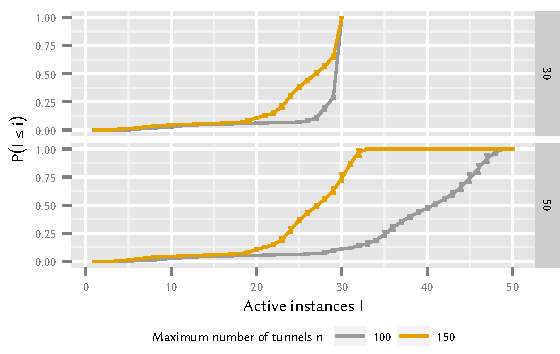
\includegraphics{cloud/virtualized_network_functions/performance_evaluation/figures/instanceuse_multiserver}
  \caption{Impact of the maximum number of tunnels \(n\) and number of servers \maxServers on number of active servers in the virtual \headershortacr{GGSN} model.}
  \label{fig:cloud:virtualized_network_functions:performance_evaluation:virtual_ggsn:instanceuse_multiserver}
\end{figure}

In \reffig{fig:cloud:virtualized_network_functions:performance_evaluation:virtual_ggsn:instanceuse_multiserver} the \gls{CDF} of the number of active servers for four different virtual \gls{GGSN} configurations is displayed.
We study the behaviour of a virtual \gls{GGSN} with \(\maxServers = 30\) servers, where each server can support \(n = 100\) or \(n = 150\) tunnels.
Then, we compare this with a virtual \gls{GGSN} with \(\maxServers = 50\) servers and again \(n = 75\) or \(n = 150\) tunnels.
We observe that increasing the number of supported tunnels \(n\) per server allows a larger percentage of servers to be shut-down or used for other tasks. This demonstrates the scaling capability of the virtualised model quite well.
Note that both the scenario with \(30\) servers \maxServers and \(150\) maximum tunnels \(n\) per server as well as the scenario with \(60\) servers \maxServers and \(75\) maximum tunnels per server sharing the same maximum amount of tunnels, i.e. \(4500\), being right at the centre of the interesting range of candidates.

\begin{figure}
  \centering
  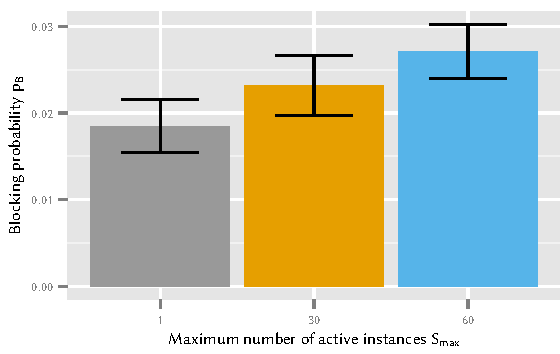
\includegraphics{cloud/virtualized_network_functions/performance_evaluation/figures/blocking_comparison}
  \caption{Impact of blocking probability \blockingprobability on the number of servers compared to the traditional \headershortacr{GGSN}, \(4500\) maximum tunnels per server being on a single server, i.e. \(150\) on \(30\), and \(75\) on \(60\) servers.}
  \label{fig:cloud:virtualized_network_functions:performance_evaluation:virtual_ggsn:blocking_comparison}
\end{figure}

Next, we study the blocking probability of the virtual \gls{GGSN} system in \reffig{fig:cloud:virtualized_network_functions:performance_evaluation:virtual_ggsn:blocking_comparison} and compare it to the results from the traditional \gls{GGSN} model with both systems dimensioned for \(4500\) tunnels.
We observe that, considering the start-up and shut-down time of \SI{300}{\second}, the blocking probability \blockingprobability increases by a factor of \(1.46\) if the virtual \gls{GGSN} is comprised of \(60\) instances \(\maxServers\) dimensioned for \(75\) concurrent tunnels \(n\) , i.e. \(\frac{1}{60}\) of the original server capacity.
In this case \(27\) of all \(60\) servers can be turned off or used for other purposes at \SI{50}{\percent} of the time.
We conclude that choosing more powerful servers decreases the blocking probability but reduces the potential to disable servers.

So far we have considered a conservative start-up and shut-down time of servers \(d\) of 5 minutes, which can potentially occur in non-virtualised available hardware.
In the next section we study the impact of reduced start-up and shut-down times with modern servers with fast storage, e.g. \glspl{SSD}, or containerised applications\footnote{\url{https://www.docker.com/}, \accessed}.

\subsubsection*{Impact of Start-up and Shut-down Times}\label{sec:cloud_virtualized_network_functions:startup_shutdown}

In this section, we first consider the impact of different start-up and shut-down times \(d\) on resource utilisation \(n_A\) and blocking probabilities \blockingprobability.
Afterwards, the influence of varying server start and stop times \(d\) on a fixed combination of maximum tunnels \(n\) and servers \maxServers in the system is examined.

\begin{figure}
  \centering
  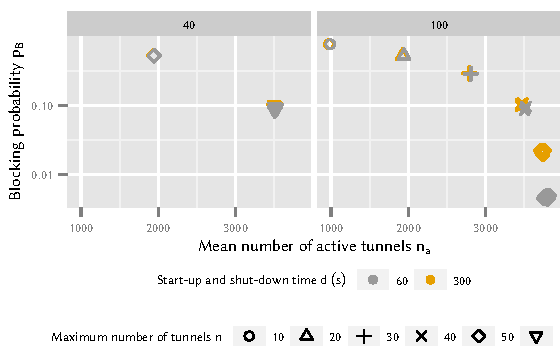
\includegraphics{cloud/virtualized_network_functions/performance_evaluation/figures/compare_util_block}
  \caption{Trade-off between blocking probability \blockingprobability and mean resource utilisation \(n_A\) with regard to maximum number of instances \maxServers, maximum number of tunnels per server \(n\), and start-up and shut-down time \(d\).}
  \label{fig:cloud_virtualized_network_functions:startup_shutdown:compare_util_block}
\end{figure}

\reffig{fig:cloud_virtualized_network_functions:startup_shutdown:compare_util_block} shows scenarios with \(40\) and \(100\) \gls{GGSN} instances \(maxServers\) and  \(1000\) to \(5000\) total concurrent tunnels.
For each scenario, we study the impact of selecting a different maximum number of tunnels \(n\) per server as well as start-up and shut-down times \(d\) on blocking probability \blockingprobability and mean resource utilisation \(n_A\).
The first observation is that by increasing the number of servers \(\maxServers\), i.e. scaling out, the blocking probability \blockingprobability can be decreased, while maintaining a relatively low mean resource utilisation \(n_A\).
In addition to the previous effects, we notice that a higher start-up and shut-down time \(d\) causes a slight increase in blocking probability \blockingprobability for servers with low tunnel capacity \(n\).

\begin{figure}
  \centering
  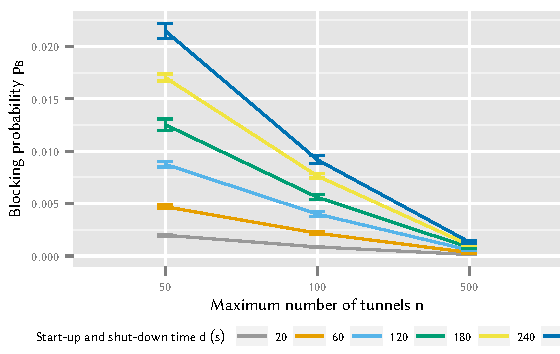
\includegraphics{cloud/virtualized_network_functions/performance_evaluation/figures/compare_maxinstances_block}
  \caption{Influence of start-up and shut-down time \(d\) on blocking probability \(p_B\) with regard to different numbers of supported tunnels per instance \(n\).}
  \label{fig:cloud_virtualized_network_functions:startup_shutdown:compare_maxinstances_block}
\end{figure}

We focus on a specific scenario in \reffig{fig:cloud_virtualized_network_functions:startup_shutdown:compare_maxinstances_block}, where \(5000\) total tunnels should be supported by the system, to study this behaviour in more detail.
To achieve this goal, we consider three types of instances, with the server capacity \(n\) varying between \(50\) and \(500\).
In each case we change the start-up and shut-down time \(d\) between \(20\) and \(\SI{300}{\second}\).
We observe that lower server capacities \(n\) combined with higher start-up and shut-down times \(d\) increase the blocking probability \blockingprobability.
This is due to the server start-up threshold mechanism, used in the model, not taking the additional capacity gained by activating an additional server into account.
If a low capacity server with a long boot time is activated, there is a high probability that the system will quickly expend its capacity again.

Thus, it can be concluded that if smaller instances are to be used, e.g. due to the fact that they are cheaper than large instances, start-up and shut-down times should be kept minimal, for example by using containers or \glspl{SSD}.

\subsection{Impact of Application Traffic Patterns}\label{sec:network:network_traces:numerical_results}
In the measurement study, we apply the methods introduced in \refsec{sec:network:network_traces:performance_evaluation} to four popular smartphone
applications to infer signalling traffic and power drain.
First, we characterise the applications in terms of traffic patterns, application usage, as well as bandwidth requirements.
Then, we study the \gls{SF} and power drain caused by these applications if the inactivity timers, i.e. \TDCH or \TFACH are modified.
Finally, we analyse the influence of network parameters on web \gls{QoE} in terms of \gls{MOS} depending on page load times which are influenced by the network settings.

\subsubsection*{Characterisation of Traffic Patterns for Selected Applications}\label{sec:network:network_traces:numerical_results:traffic_characterization}

\begin{table}
  \centering
  \caption{Qualitative characterization of applications under study.}
  \label{tab:network:network_traces:numerical_results:app_characterization}
  \begin{tabular}{lccc}
  	\toprule
    Application&Traffic&Application&Required\\
    &characteristic&use&bandwidth\\
    \midrule
    Angry Birds & Interactive & Foreground & Low bandwidth \\
    Aupeo & Interactive & Background & High bandwidth\\
    Twitter & Periodic, Low frequency & Background & Low bandwidth\\
    Skype & Periodic, High frequency& Background & Low bandwidth\\
    \bottomrule
  \end{tabular}
\end{table}

For this study we chose four specific applications in order to cover a broad spectrum of traffic characteristics, as described in \reftab{tab:network:network_traces:numerical_results:app_characterization}.
First, we discuss said characteristics for these applications.
We differentiate between applications, where the user interaction causes the generation of traffic, and those, where the application periodically sends or receives traffic.
Finally, we consider the amount of bandwidth used by the application.

\textbf{Angry Birds} for Android is a popular \emph{interactive} free-to-play game and runs in the \emph{foreground}.
To finance the game, an advertisement is shown once the player starts or restarts a level.
Advertisements are downloaded on demand by the application, but require \emph{low bandwidth}.
Thus, the time between two advertisements depends on the frequency of the player advancing to the next level or deciding to restart the current one.

\textbf{Aupeo} is an Internet radio application, allowing a user to listen to content from personalised radio stations, while running in the \emph{background}.
Content is not streamed but downloaded at the beginning of the track.
The exact duration depends on the radio stations chosen by the user and is thus \emph{interactive}.
This results in large times of inactivity during the playback of the track itself.
Due to the fact that audio files are downloaded, there is a \emph{high bandwidth} requirement.

The \textbf{Twitter} client is used to send and receive new short messages from the user's Twitter account.
Transferring these messages requires relatively \emph{low bandwidth}.
To this end, the user can specify an update frequency when to pull new messages in the \emph{background}.
Thus, the downloads occur with a \emph{periodic behaviour of low frequency}, where
the client sends an \gls{HTTPS} request to the Twitter server and in return receives new Tweets for the user's account.
We do not consider an active user who is publishing new Tweets.
Such behaviour would manifest as additional traffic to the periodic one generated by the status updates.
Due to the fact that publishing updates occurs relatively infrequently, and updating the feed occurs more often, the traffic generated by publishing updates is dominated by that occurring due to updates, and thus can be neglected.

Finally, we consider the \textbf{Skype} application.
We do not consider any \gls{VoIP} calls, but the application's idle behaviour, i.e. when the application is running in the \emph{background}.
During this time, the application sends keep-alive messages to the network.
These keep-alive messages are sent with a \emph{high frequency} and require \emph{low bandwidth}.

In addition to the applications considered, there exist other categories of applications which are running in the \emph{foreground} and \emph{interactively} require a \emph{high bandwidth}.
One example for such an application is Skype while taking a \gls{VoIP} call.
These applications are not considered in this study, as this kind of behaviour causes the \gls{UE} to be always online.
This results in the minimal amount of signalling messages to be sent and a maximal power drain at the \gls{UE}, independent of network model or used parameters.
Other combinations of traffic criteria also exist.
However, from both, a signalling frequency as well as a power drain point of view, they can be mapped to one of the discussed cases.
For example, if an application is sending periodic updates with low bandwidth without user interaction, then the fact that the application is running in the foreground or the background is without consequence for the generated signalling frequency or power drain.
However, these cases should be considered when optimisation strategies for message sending are under study.
Background applications, for instance, could allow for the batching of messages, due to the fact that the transmission is usually not urgent, while foreground applications do not allow for such behaviour as it would delay the user interactions and consequently decrease \gls{QoE}.

Next, we describe the applications under study in more detail.
For each application we show the \gls{CDF} of the inter-arrival times in \reffig{fig:network:network_traces:numerical_results:traffic:interarrival_times} and give information about the mean values and standard deviation of both inter-arrival times and bandwidth in \reftab{tab:network:network_traces:numerical_results:traffic_statistics}, respectively.

\begin{figure}
\centering
\includegraphics{network/network_traces/numerical_results/figures/interarrival_times}
\caption{\headershortacr{CDF} of inter-arrival times for considered applications.}\label{fig:network:network_traces:numerical_results:traffic:interarrival_times}
\end{figure}

\begin{table}
  \centering
  \caption{Mean and standard deviation of inter-arrival time and bandwidth for considered applications.}
  \label{tab:network:network_traces:numerical_results:traffic_statistics}
  \begin{tabular}{lcccc}
  	\toprule
    Application&\multicolumn{2}{c}{Inter-arrival time (\si{\second})}&\multicolumn{2}{c}{Bandwidth (\si{\kilo\bit\per\second})}\\
    \cmidrule(lr){2-3}\cmidrule(lr){4-5}
    &Mean&Standard deviation&Mean&Standard deviation\\
    \midrule
    Angry Birds&0.66 &15.90 & 4.42 & 4.50\\
    Aupeo&0.06 & 3.06& 129.76 & 482.63\\
    Twitter& 8.91&44.09 & 0.27 & 0.04\\
    Skype& 0.55 &1.95 & 1.30 & 1.84\\
    \bottomrule
  \end{tabular}
\end{table}

\begin{enumerate}
\item \textbf{Angry Birds}
We see that there are no distinct peaks in inter-arrival time, which would indicate a periodic behaviour.
Furthermore, we see that \SI{5}{\percent} of all inter-arrival times are greater than \SI{1}{\second}.
As we consider only \TDCH values above \SI{1}{\second}, those are candidates for triggering state transitions.
The mean inter-arrival time is \SI{0.66}{\second}, with a relatively high standard deviation of \SI{15.90}{\second}.
This is caused by the low inter-arrival times in one advertisement request at the beginning of each new level and the relatively large inter-arrival times between two advertisements.
Mean bandwidth is relatively low with \SI{4.42}{\kilo\bit\per\second} and a high standard deviation of \SI{4.5}{\kilo\bit\per\second}.
These differences can be explained by considering the behaviour of the application.
During long phases of use no traffic is sent, and after a level is restarted, a new advertisement has to be obtained, causing the transmission of data.
Note that no level data is downloaded during gameplay at all, as the complete game is downloaded during the installation process.

\item \textbf{Aupeo} We see that the application generates packets with relatively small inter-arrival times with a small mean inter-arrival time of \SI{0.06}{\second}.
The high standard deviation of \SI{3.06}{\second} is caused by the waiting between two tracks.
Furthermore, we see a high mean bandwidth of \SI{129.76}{\kilo\bit\per\second}, and a standard deviation of \SI{482.63}{\kilo\bit\per\second}.
This is caused by the difference in traffic activity between times when tracks are either downloaded or not.

\item \textbf{Twitter} We see that \SI{90}{\percent} of all transmissions occur with an inter-arrival time of less than \SI{1}{\second}.
Also, we can observe a high mean inter-arrival time of \SI{8.91}{\second} and a high standard deviation of \SI{44.49}{\second}.
Additionally, the mean bandwidth is low with only \SI{0.27}{\kilo\bit\per\second} and a low standard deviation of \SI{0.04}{\kilo\bit\per\second} due to the fact that Twitter text messages are only \(140\) characters in length and thus only a low volume of traffic needs to be transmitted.

\item \textbf{Skype} Similar to the Twitter application, we see that \SI{90}{\%} of all packets occur with an inter-arrival time of less than \SI{1}{\second}.
However, in contrast to Twitter, we see a low mean inter-arrival time of \SI{0.55}{\second} with a standard deviation of \SI{1.95}{\second}.
Further, we observe a relatively low mean bandwidth of \SI{1.30}{\kilo\bit\per\second} and a standard deviation of \SI{1.8}{\kilo\bit\per\second}.
\end{enumerate}

\begin{figure}
\centering
\includegraphics{network/network_traces/numerical_results/figures/autocorrelation}
\caption{Autocorrelation of inter-arrival times for considered applications.}\label{fig:network:network_traces:numerical_results:traffic:autocorrelation}
\end{figure}

To further study the traffic patterns of the applications, we study the autocorrelation of the packet inter-arrival time with regard to the lag length in \reffig{fig:network:network_traces:numerical_results:traffic:autocorrelation}.
We note that all studied applications present completely different autocorrelations for the inter-arrival times.
This is one of the reasons that the applications under consideration will display different signalling behaviour in the next section.

\subsubsection*{Influence of Application Characteristics on Optimisation with Network Timers}\label{sec:network:network_traces:numerical_results:application_influence}
This section studies the impact of traffic generated by applications on both the network and the
\gls{QoE} of the user.
We consider two metrics.
First, we consider the frequency of signalling messages induced at network components in the \gls{RAN}.
In light of network outages caused by so called signalling storms, a large number of signalling messages leading to overload at network equipment, it is in the interest of a network operator to reduce the number of signalling messages arriving at the \gls{RNC}.
One possible way to reduce the signalling frequency \gls{SF} is to modify network timer values, i.e., \TDCH and \TFACH.

As discussed in \refsec{sec:network:background:energy_consumption_qoe}, the \gls{QoE} a user perceives while using the device is influenced by the battery life of the \gls{UE}.
Thus, the second metric considered is the device’s power drain which is influenced by the used network model and associated timer settings.
As described in \refsec{sec:network:network_traces:calculating_metrics}, based on a measurement trace for an application we use \refalg{alg:network:network_traces:performance_evaluation:inferring_network_state:inference_algorithm} to infer the state transitions occurring during the use of the application.
Then, we calculate the relative time spent in each state and use \reftab{tab:network:network_traces:calculating_metrics:power_consumption} to compute the mean power
drain of the radio interface during the measurement.
We study both metrics, first on their own and then aggregated for both network models introduced in \refsec{sec:network:background:umts_rrc}.

In this section we first consider the Three State Model, which describes the default behaviour in \gls{3G} networks.
Then, we describe the influence of the Two State Model which models a network behaviour similar to that if proprietary fast dormancy algorithms are used.
These algorithms have been identified as one of the causes of a signalling storm~\cite{NSN2011}.
Finally, we summarise the results and discuss the possible ramifications of using network timer values to reduce the signalling frequency.

\paragraph*{Three State Model: Signalling Frequency vs. Power Consumption}\label{sec:network:network_traces:numerical_results:three_states}
First, we investigate the signalling frequencies generated by the studied applications for the Three State Model.
\reffig{fig:network:network_traces:numerical_results:three_states:three_states:signalling} shows the signalling frequency \gls{SF} with regard to the \TDCH timer.
\begin{figure}
	\centering
	\includegraphics{network/network_traces/numerical_results/figures/3_state_tdch_vs_frequency}
	\caption{Signalling frequency \headershortacr{SF} for varying \TDCH timers for the Three State Model.}\label{fig:network:network_traces:numerical_results:three_states:three_states:signalling}
\end{figure}
For all studies of the Three State Model, the \TFACH timeout is set to \(\TFACH = 2\cdot  \TDCH\), a realistic value as shown in \cite{Qian2011a}.
We see that for \TDCH timers shorter than \SI{6}{\second} the Skype application in \gls{RRC_idle} mode generates the highest signalling frequency.
The Angry Birds application generates the second highest frequency of signalling messages, followed by the Aupeo application.
The Twitter application generates the smallest signalling frequency.
If the \TDCH value is longer than \SI{15}{\second}, this order changes.
However, in general the signalling frequency for higher \TDCH timeouts is lower than for shorter \TDCH timeouts.
Now, the Aupeo application has the highest signalling frequency, followed by the Twitter application.
The signalling frequency for the Angry Birds application takes the third place.
The application which generated the highest signalling frequency generates the lowest frequency for higher timeout values.
This behaviour can be explained by the fact that the Skype application sends keep-alive messages with an interval of less than \SI{20}{\second}.
If the timer is greater than the interval time of the keep-alive messages, the \gls{UE} stays always connected and thus generates almost no signalling.

These results show that the traffic patterns of the application have a large influence on the generated signalling frequency.
Signalling is generated for every pause in sending or receiving larger than the configured timeouts.
If such pauses occur frequently, this increases the signalling frequency as shown on the examples of Skype and Angry Birds.
Applications with more time between sending or receiving of data cause less signalling, as shown by Aupeo and Twitter.
Furthermore, we can observe that the signalling frequency can be reduced by increasing the \TDCH timeout, with the minimum being reached as \TDCH approaches infinity.
From a signalling frequency perspective, a value of \SI{20}{\second} would probably be sufficient, however if other metrics, e.g. radio resource consumption, are considered \SI{10}{\second} would be acceptable for a network operator.

Based on this finding, we see that increasing the \TDCH timer decreases the signalling frequency \gls{SF} at the \gls{RNC}.
However, the actual signalling frequency depends on the application running at the \gls{UE}.
From a network operator's point of view, the Three State Model should always be preferred to the Two State Model as it generates less signalling messages per second, thus decreasing the load at the \gls{RNC}.
This view does however not consider the additional radio resources which are kept in use for a longer time if larger \TDCH values are used.
Additionally, it should be noted that the choice of the network model is sometimes outside of the domain of the network operator.
Proprietary Fast Dormancy algorithms, as the considered Two State Model, are enabled on the \gls{UE} by the user.

\begin{figure}
	\centering
	\includegraphics{network/network_traces/numerical_results/figures/3_state_tdch_vs_power_drain}
	\caption{Power drain \headershortacr{PD} for varying \TDCH timers for the Three State Model.}\label{fig:network:network_traces:numerical_results:three_states:power_drain}
\end{figure}
In \reffig{fig:network:network_traces:numerical_results:three_states:power_drain} we consider the power drain if the network uses the Three State Model, i.e. if the Fast Dormancy mode of the \gls{UE} is disabled.
The figure shows the mean power drain \gls{PD} of the device with regard to the \TDCH timeout.
Possible values range between \SI{0}{\milli\watt}, if the \gls{UE} was in \gls{RRC_idle} state during the whole measurement, and \SI{800}{\milli\watt}, if the \gls{UE} was in \gls{RRC_DCH} state during the complete measurement.
We see that the lowest power over all considered \TDCH values is consumed by the Twitter application.
The second least power drain is required by Aupeo, followed by Angry Birds.
Finally, the most power is consumed by Skype.
Here we see that the maximum value of \SI{800}{\milli\watt} is reached at a \TDCH timeout of \SI{20}{\second}.
Due to the periodic traffic behaviour of Skype, the device is always in \gls{RRC_DCH} state.
Again we see that the traffic characteristics of the applications impact the power drain.
Applications with more network activity are forced to stay in connection states requring a larger amount of power for a longer time.
We see that for very small network timers, the power drain is minimal.
However, as seen in the last section small timers increase the signalling frequency at the \gls{RNC}.
Again, a choice of \SI{10}{\second} for the \TDCH timer can be seen as a compromise between signalling frequency \gls{SF} and power drain \gls{PD}.

\begin{figure}
	\centering
	\includegraphics{network/network_traces/numerical_results/figures/3_state_signalling_vs_power_consumption}
	\caption{Influence of manipulating \TDCH timer on signalling frequency \headershortacr{SF} and power drain \headershortacr{PD} for the Three State Model. Filled marker highlights \(\TDCH = \SI{11}{\second}\).}\label{fig:network:network_traces:numerical_results:three_states:trade_off}
\end{figure}
Finally, we aggregate both metrics in in \reffig{fig:network:network_traces:numerical_results:three_states:trade_off}.
The x-axis of the figure gives the signalling frequency.
On the y-axis we show the power drain \gls{PD}.
Different \TDCH values are shown by different colours as specified by the colour bar.
First, we consider Angry Birds.
We observe that as the signalling frequency approaches zero, the power drain rapidly increases, even if only small gains in signalling frequency reduction can be achieved.
The Aupeo application presents a completely different picture.
Here, we can see multiple almost horizontal lines of markers.
If \TDCH is chosen in this range, each increase of \TDCH brings a small decrease in signalling frequency \gls{SF} for an increase in power drain \gls{PD}.
However, some points of discontinuity exist.
If for example the \gls{RRC_DCH} timer is increased from \SI{10}{\second} to \SI{11}{\second}, a decrease in signalling frequency \gls{SF} of \SI{40}{\percent} can be achieved by only suffering from a small increase in power drain.
These points of discontinuity would present themselves to be suitable targets of optimisation.
Next, we consider the Twitter application.
It displays a similar behaviour as the Aupeo application, with multiple points of discontinuity.
Note that Twitter exhibits a different point of discontinuity, and the \TDCH value of \SI{10}{\second}, which provided good results for Aupeo, is not optimal for Twitter.
Finally, Skype again shows a completely different picture than all the other considered applications.
First, note that due to the large signalling frequency \gls{SF} of Skype for small values of \TDCH, \(\TDCH = \SI{1}{\second}\) is not displayed in the figure.
Furthermore, as the \TDCH timer increases above \SI{20}{\second} the signalling frequency \gls{SF} does not decrease any further, and the power drain \gls{PD} remains at the maximum value.
We observe that there is no common optimal value for all applications which would result in an acceptable tradeoff.


\paragraph*{Two State Model: Signalling Frequency vs. Power Drain}\label{sec:network:network_traces:numerical_results:two_states}
Now, we study the consequences of the application traffic in a network using the Two State Model.
The Two State Model occurs in reality if Fast Dormancy implementations are considered.
Here, the \gls{UE} disconnects from the network if for a certain time no traffic is sent or received in order to reduce power drain.
\begin{figure}
	\centering
	\includegraphics{network/network_traces/numerical_results/figures/2_state_tdch_vs_frequency}
	\caption{Signalling frequency \headershortacr{SF} for varying \TDCH timers for the Two State Model.}\label{fig:network:network_traces:numerical_results:two_states:signalling}
\end{figure}
As for the Three State Model, \reffig{fig:network:network_traces:numerical_results:two_states:signalling} shows the signalling frequency \gls{SF} with regard to the setting of the \TDCH timer.
We see the same general behaviour as with the Three State Model, however the signalling frequencies generated by each of the applications for the Two State Model are usually higher.
For example, even for relatively high \TDCH timeout values of \SI{10}{\second}, the Angry Birds application causes \SI{270}{\percent} of the signalling frequency \gls{SF} with respect to a network using the Three State Model.

\begin{figure}
	\centering
	\includegraphics{network/network_traces/numerical_results/figures/2_state_tdch_vs_power_drain}
	\caption{Power drain \headershortacr{PD} for varying \TDCH timers for the Two State Model.}\label{fig:network:network_traces:numerical_results:two_states:power_drain}
\end{figure}
Next, we consider the changes in the power drain of the \gls{UE} if the user decides to enable Fast Dormancy, i.e. switch to a Two State Model, in \reffig{fig:network:network_traces:numerical_results:two_states:power_drain}.
As with the signalling frequency, we only see a quantitative difference to the Three State Model.
Again, we compare the differences between Two State Model and Three State Model on the example of the Angry Birds application.
For the same considered \TDCH timeout of \SI{10}{\second}, we see a decrease of \SI{81}{\percent} in power drain \gls{PD} when compared with the Three State Model.

\begin{figure}
	\centering
	\includegraphics{network/network_traces/numerical_results/figures/2_state_signalling_vs_power_consumption}
	\caption{Influence of manipulating \TDCH timer on signalling frequency \headershortacr{SF} and Power drain \headershortacr{PD} for the Two State Model. Filled marker highlights \(\TDCH = \SI{11}{\second}\).}\label{fig:network:network_traces:numerical_results:two_states:trade_off}
\end{figure}
Finally, we compare the influence of changes of the \TDCH timeout on both signalling frequency \gls{SF} and power drain \gls{PD} for the Two State Model in \reffig{fig:network:network_traces:numerical_results:two_states:trade_off}.
As for the Three State Model, we see that there is no tradeoff between power drain and signalling frequency which would be acceptable for all application.
Even for single applications \TDCH values, as for example the earlier discussed \SI{10}{\second}, which for Angry Birds was an acceptable tradeoff, is no longer a good choice in the Two State Model.

\subsubsection*{Consequences of Trade-Off: Signalling Frequency vs. Power Drain}\label{sec:network:network_traces:numerical_results:trade_off}

In order to illustrate the impact of the behaviour discussed in the previous section, we compare the influence of the \TDCH timer on two applications with different traffic characteristics in  \reffig{fig:network:network_traces:numerical_results:consequences}.

\begin{figure}
	\begin{subfigure}[b]{.5\textwidth}
	\centering
	\includegraphics{network/network_traces/numerical_results/figures/consequences_aupeo}
	\caption{Aupeo}\label{fig:network:network_traces:numerical_results:consequences:aupeo}
	\end{subfigure}
	\begin{subfigure}[b]{.5\textwidth}
	\centering
	\includegraphics{network/network_traces/numerical_results/figures/consequences_angry_birds}
	\caption{Angry Birds}\label{fig:network:network_traces:numerical_results:consequences:angry_birds}
	\end{subfigure}
	\caption{Influence of manipulating \TDCH timer on different applications.}\label{fig:network:network_traces:numerical_results:consequences}
\end{figure}

First, we consider the Aupeo application as shown in \reffig{fig:network:network_traces:numerical_results:consequences:aupeo}.
The signalling frequency \gls{SF} before the increase of the \TDCH timer was \(0.55\) messages per second, after the change to \(\TDCH = \SI{8}{\second}\) the signalling frequency remains unchanged.
Thus, the policy change based on one application brings no significant gain to other applications.
However, from a user's point of view, the power drain \gls{PD} increased from \SI{121}{\milli\watt} to \SI{183}{\milli\watt}.
Again, we assume the user activates fast dormancy to deal with the increase in power drain of more than $50\%$.
This results in a decrease of power drain \gls{PD} to \SI{117}{\milli\watt}, and an increase of overall signalling frequency \gls{SF} to \(0.76\) messages per second.
By changing the value without considering all applications, the network operator reduces the \gls{QoE} for other users, and worsens the overall situation.
Thus, due to the large number of applications it seems impossible to optimise the \TDCH timeout to reduce the signalling frequency without negatively impacting the users \gls{QoE} in unexpected ways.
The Angry Birds application shown in  \reffig{fig:network:network_traces:numerical_results:consequences:angry_birds} shows quantitatively similar results.

There exist applications, like Twitter and Aupeo, where optimisation by modifying the \TDCH values can provide acceptable results.
However, these optimisations are only successful if a single application or network model is considered.
For other applications, like Angry Birds or Skype, this optimisation approach does not seem to be successful.
A reduction of signalling frequency and power drain is possible, if the application developers are incentivised to optimise their applications accordingly.
In \cite{Qian2011a} the authors suggest methods to achieve this optimisation, for example batch transfer of advertisements for applications like Angry Birds or decreasing the refresh rate in applications like Skype.
However, at the moment application developers are neither receiving incentives to optimise applications in this way, nor do hardware vendors provide interfaces to facilitate such optimisation.
Such interfaces would allow application developers to schedule their data transmissions in such a way that both signalling and battery drain would be reduced.
Additionally, these interfaces would need to allow the application developer to specify whether sending the transmission is urgent.
One example of such urgency would be if the application is being actively used by the user and requires the feedback of the transmission.
If the data is being sent as a regular update while the application is running in the background it could be scheduled for later transmission as suggested by \cite{Calder2010, Vergara2012}.

\subsection{Influence of Network Configuration and Background Traffic on Web \headershortacr{QoE}}\label{sec:network:network_traces:numerical_results:web_qoe}
So far we have discussed only power drain as a \gls{QoE} influence factor.
For applications like web browsing, one relevant QoE influence factor are page load times.
Therefore, we consider a web QoE model which quantifies the impact of page load times on mean opinion scores \cite{egger2012a}.
Here we distinguish between \emph{web \gls{QoE}} and \emph{\gls{QoE}}, as no \gls{QoE} models are currently existing which consider page load times as well as power drain.
In this section, we study the impact of background traffic as well as network timer settings on the page load time of an image and the resulting \gls{MOS}.
For this study, we only consider the Three State Model, but the results can be applied to the Two State Model as well.

We assume a scenario, where a user is running a background application like Twitter or Skype.
Then, while the application is in the background, the user begins to download an image from a website.
Due to the background traffic, and depending on the network model and associated timer values, the \gls{UE} may be currently either in \gls{RRC_idle}, \gls{RRC_FACH} or \gls{RRC_DCH} state.
We give the probability of a random observer encountering the system in \gls{RRC_FACH} state by \(p_{\gls{RRC_FACH}}\) and the probability of a random observer encountering in \gls{RRC_idle} state by $p_{\gls{RRC_idle}}$.
If the device is currently not in \gls{RRC_DCH} state, it takes some time to connect.
This promotion time depends on the current state and is according to \cite{Qian2010b} \SI{2.5}{\second} if the \gls{UE} is in \gls{RRC_idle} state and \SI{1.5}{\second} if the device is in \gls{RRC_FACH} state.
For this study, we assume that the user randomly chooses a time to begin downloading an image.
The time until the image is displayed consists of the time to load the page \(t_p\), as well as the time to go online \(t_o\), where \(t_o\) is the mean time to go online, given as
\[t_o = p_{\gls{RRC_idle}} \cdot \SI{2.5}{\second} + p_{\gls{RRC_FACH}} \cdot \SI{1.5}{\second}.\]
In reality, an additional delay is added due to the latency of the physical display, however as this happens in a smaller timescale we neglect it in this model.
Thus, the total time \(t\) that is required to download the image is given by \(t = t_o + t_p\).

The authors of \cite{egger2012a} give a function to calculate the \gls{MOS} based on the required page load time as \(QoE(t) = a\cdot \ln t + b\), were \(a\) and \(b\) depend on the type of content being downloaded.
For our scenario, picture download, values of \(a = -0.8\) and \(b = 3.77\) are suggested.
It has to be noted that for different web sites, the logarithmic function was still observed, but different values for \(a\) and \(b\) were obtained as given in \cite{egger2012a}.
These values depend for example on the type of web page as well as the size of the content.
Nevertheless, the results presented in this section are therefore generalisable for web browsing to various pages.
This allows us to give an expected \gls{MOS} for downloading pictures while a background application is influencing the probability of a device already being in \gls{RRC_DCH} state or still having to be promoted to \gls{RRC_DCH} state.

\begin{figure}
	\begin{subfigure}[b]{\textwidth}
	\centering
	\includegraphics{network/network_traces/numerical_results/figures/qoe_with_backgroundapp_twitter}
	\caption{Background traffic generated by Twitter.}\label{fig:network:network_traces:numerical_results:web_qoe:twitter}
	\end{subfigure}

	\begin{subfigure}[b]{\textwidth}
	\centering
	\includegraphics{network/network_traces/numerical_results/figures/qoe_with_backgroundapp_skype}
	\caption{Background traffic generated by Skype.}\label{fig:network:network_traces:numerical_results:web_qoe:skype}
	\end{subfigure}

	\caption{Perceived web \headershortacr{QoE} for loading a page with existing background traffic.}\label{fig:network:network_traces:numerical_results:web_qoe}
\end{figure}

Using this methodology, we study the influence of background traffic on the \gls{QoE} for two background applications with different traffic characteristics.
In \reffig{fig:network:network_traces:numerical_results:web_qoe:twitter} we assume that the user is running the Twitter application as a background process.
The application is set to update the user's status feed every \SI{300}{\second}.
In \reffig{fig:network:network_traces:numerical_results:web_qoe:skype} the user is running the Skype application as a background application.
This application sends keep alive messages every \SI{20}{\second}.
For each application, we assume the Three State Model with \TDCH settings of \SIlist{1;4;8;16}{\second}.
We always set \(\TFACH = 2\cdot \TDCH\).
In both figures we show the assumed page load time \(t\), as provided by the network, on the x-axis for values from \SIrange{0.2}{25}{\second}.
We assume \SI{0.1}{\second} as a lower bound, as page load times lower than \SI{0.1}{\second} seconds are not distinguishable \cite{egger2012b} by humans.
The calculated \gls{MOS} values are given on the y-axis.

The picture downloads with the background traffic generated by the Twitter application result in \gls{MOS} values beginning at \(3.15\) for \(\TDCH = \SI{1}{\second}\), \(3.18\) for \(\TDCH = \SI{4}{\second}\), \(3.21\) for \(\TDCH = \SI{8}{\second}\), and \(3.27\) for \(\TDCH = \SI{16}{\second}\) respectively.
With increasing page load time, the \gls{MOS} decreases again.
This behaviour is due to the fact that the Twitter application periodically sends traffic every \SI{300}{\second}.
Then, no further activity occurs until the next refresh occurs.
In this time, the \gls{UE} transitions to \gls{RRC_idle} state.
This traffic characteristic causes a high probability of a user encountering the device in an \gls{RRC_idle} state.
Additionally, the traffic characteristics of the background application show that different \TDCH settings impact the web \gls{QoE} only marginally, resulting in the lines in the graph being grouped close together.

In contrast, downloading pictures with the Skype application generating background traffic, causes different \gls{MOS} values.
For a page load time \(t\) of \SI{0.2}{\second} the \gls{MOS} value with \(\TDCH = \SI{1}{\second}\) is \(3.49\), with \(\TDCH = \SI{4}{\second}\) we get \(3.99\), for \(\TDCH = \SI{8}{\second}\) we get a \gls{MOS} value of \(4.44\), and finally for \(\TDCH = \SI{16}{\second}\) we get \(4.99\) respectively.
We observe, that for increased page load times, the \gls{MOS} decreases.
Further, due to the high frequency of traffic sent by the Skype application  increased \gls{MOS} values occur when compared to those of the Twitter scenario.
Here, every \SI{20}{\second} traffic is sent.
This means that even for relatively low values of \(\TDCH\) the user has a high probability of encountering a state where no promotion delay is required before the actual page load time \(t\) can begin.

From these studies we can conclude that, when considering the \gls{QoE} on mobile devices, not only the page load time \(t\) caused by the network but also additional delays caused by the state of the device should be considered.
As shown on two examples, this state can be affected by other applications which are running in the background and generate traffic.


%\section{A Performance Model for \glsentryshort{3G} \glsentryshort{RRC} States}\label{sec:network:performance_model}
\section{A Performance Model for 3G RRC States}\label{sec:network:performance_model}
The algorithm introduced in \refsec{sec:network:network_traces} can be used to infer the signalling frequency, power drain, and \gls{QoE} of existing or prototyped applications.
However, in order to study the general impact of traffic in a comprehensive way, methods to derive said metrics from analytical traffic distributions are of interest.

In \refsec{sec:network:performance_model:analytical_model} we introduce a model allowing us to
analyse both theoretical and empirical traffic models.
Then, in \refsec{sec:network:performance_model:numerical_examples} we use this model to study the impact of traffic characteristic on metrics, i.e. signalling intensity and power drain.

%\section{System Dynamics in Fair Operation}\label{sec:network:performance_model:analytical_model}

%\subsubsection*{System Model}\label{sec:network:performance_model:analytical_model:system_model}


\subsection{The Case of Two Systems}\label{sec:network:performance_model:analytical_model:m_systems}

\subsection{The Case of Multiple Systems}\label{sec:network:performance_model:analytical_model:m_systems}

%\subsection{Numerical Examples and Implications on Fairness}\label{sec:aggregation:imbalanced:numerical_examples}

The cooperating system can benefit if the load is heterogeneously distributed among the systems, such that a system which is currently busy can offload to an idle system.
%To investigate the performance in heterogeneous load conditions we calculate the blocking probability $p_{b_1}$ of the observed system dependent on its load $\rho_1$ and the load on the links in the composite system $\rho' = \rho_i, i\in\{2,\ldots,m\}$.

In order to assess the potential of bandwidth aggregation of $m$ systems in heterogeneous load conditions, we study the load of the observed system $\rho_1$ and set the load of the other $m-1$ systems to the same value $\rho'$, i.e., $\rho_i=\rho',\forall i\in\{2,\dotsc,m\}$.
%As performance metric we consider the normalized received bandwidth of the observed system $E[X_{A_1}]/n_1$ and the bandwidth gain of the observed system $\omega_1$. We first investigate the impact of the impact of $\rho'$, then we investigate the number of cooperating systems $m$ for a fixed load $\rho'$.

%\begin{figure*}[tb]
%\centering
%\begin{subfigure}{.49\textwidth}
%  \centering
%  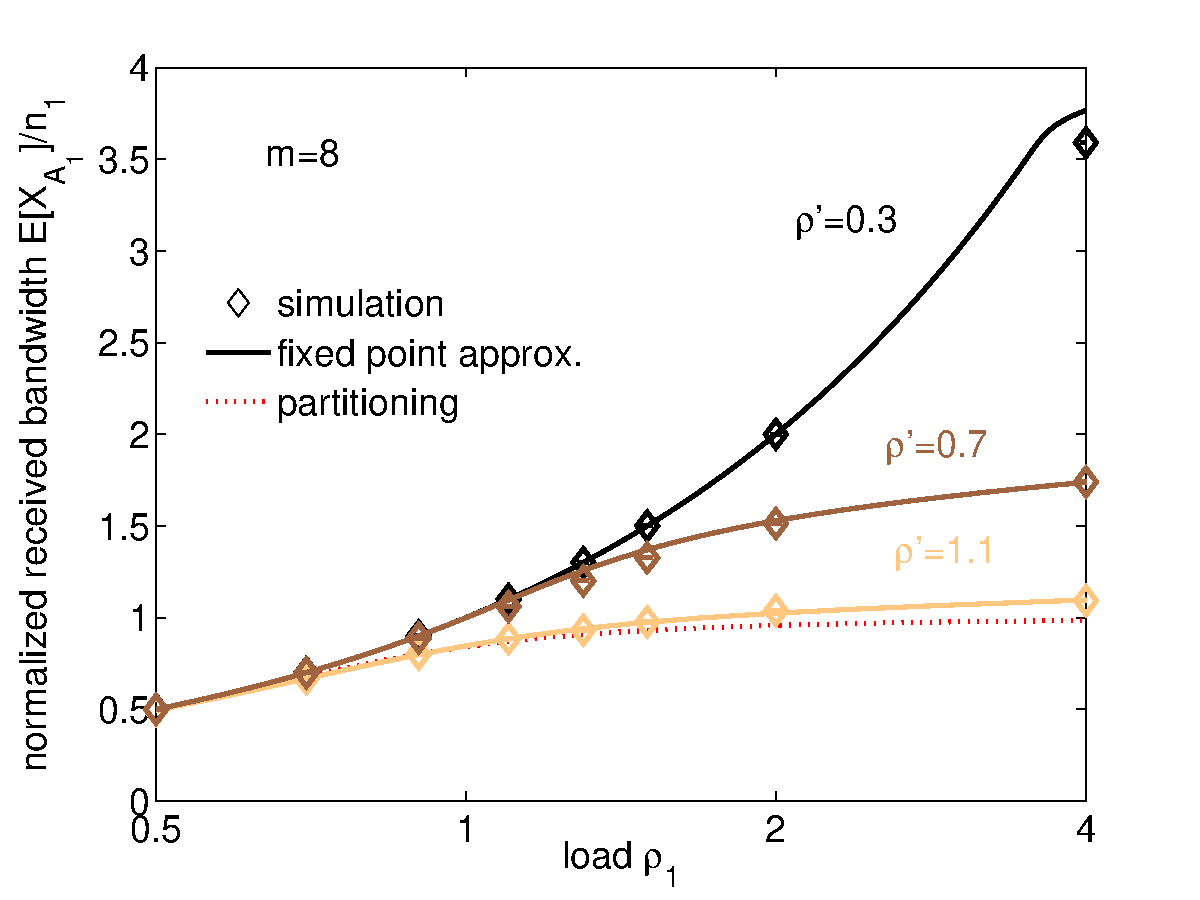
\includegraphics[width=\linewidth]{figures/fp_bw_m8}
%  \caption{Equal load}
%  \label{fig:bw_m8}
%\end{subfigure}%
%\begin{subfigure}{.49\textwidth}
%  \centering
%  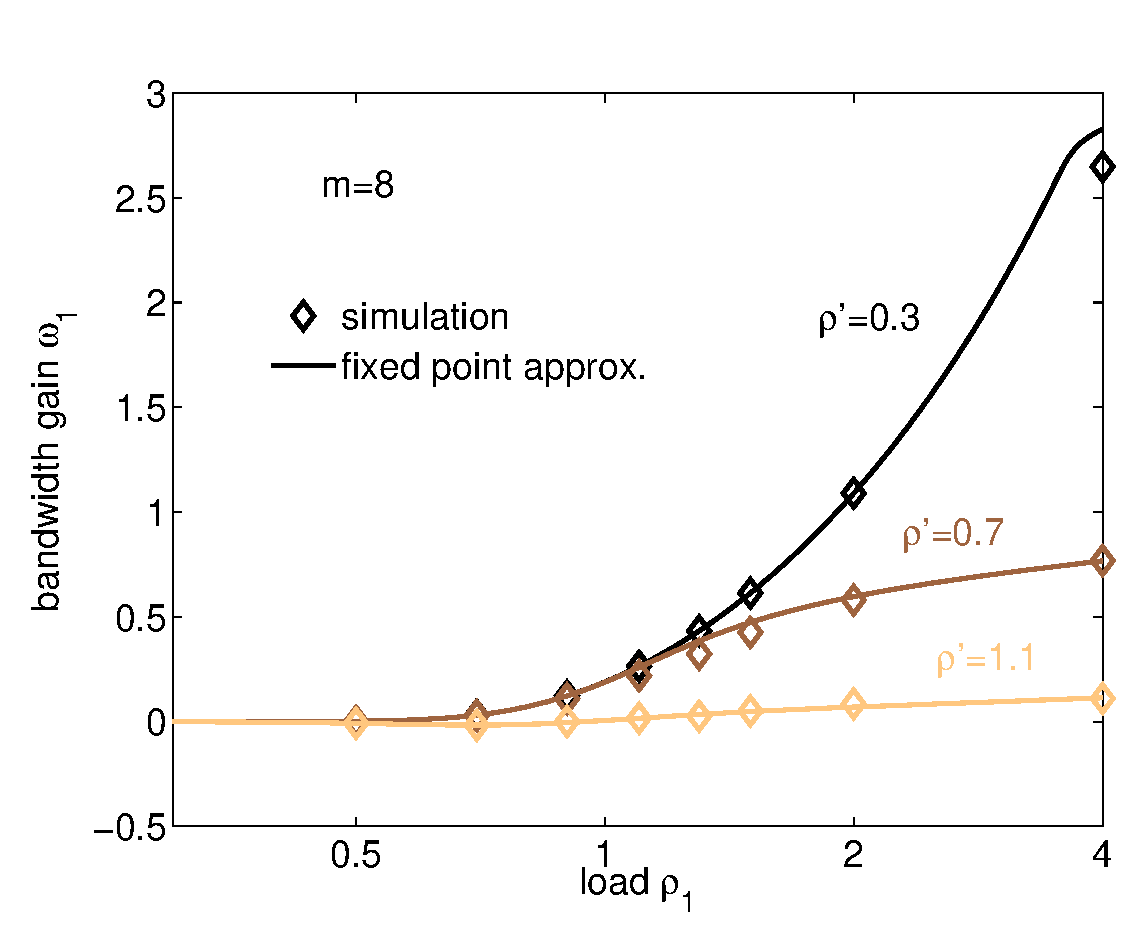
\includegraphics[width=\linewidth]{figures/fp_bwgain_m8}
%  \caption{bandwidth gain $\omega_1$}
%  \label{fig:bwgain_m8}
%  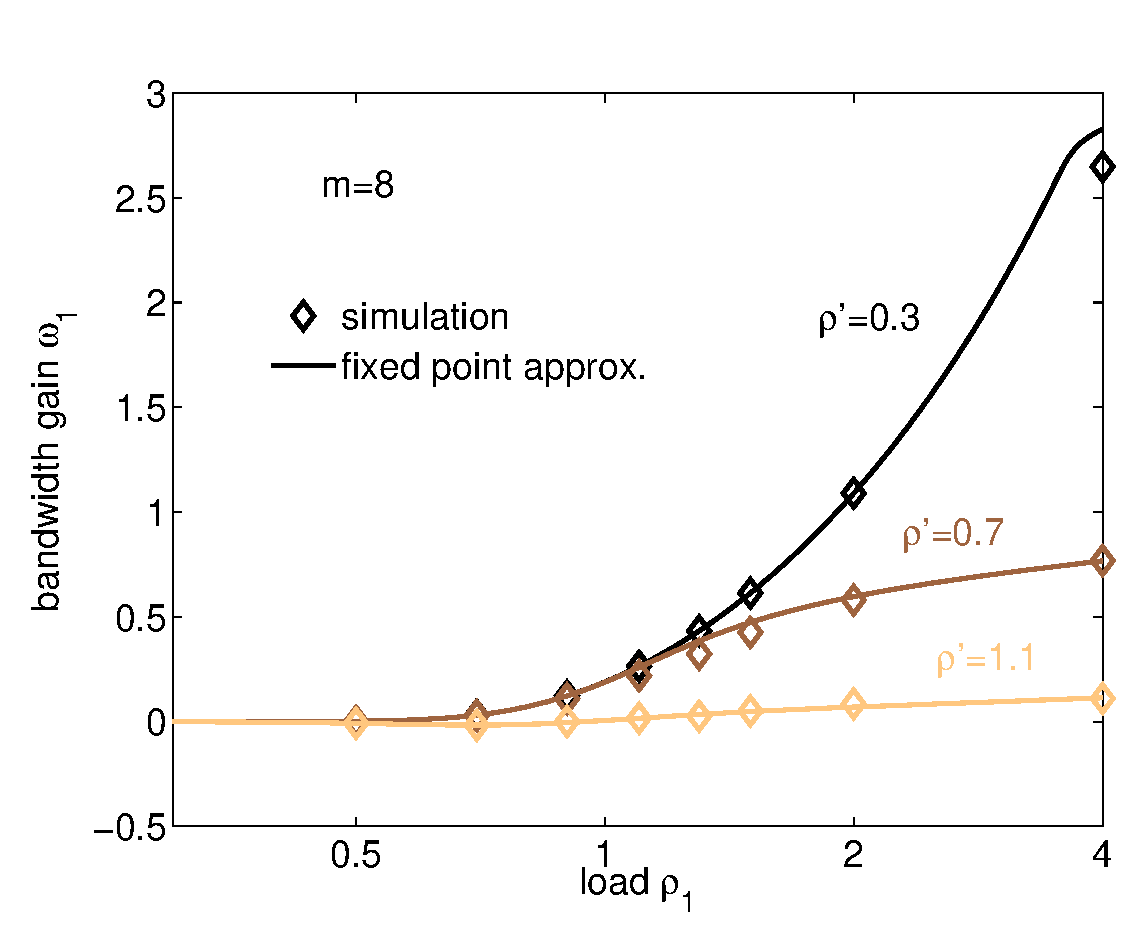
\includegraphics[width=\linewidth]{figures/fp_bwgain_m8}
%  \caption{bandwidth gain $\omega_1$}
%  \label{fig:bwgain_m8}
%\end{subfigure}
%\caption{Received bandwidth $E[X_{A_1}]/n_1$ dependent on load of the other links $\rho'$ for $m=8$}
%\label{fig:m8}
%\end{figure*}

In the following we investigate how the load on the links in the composite system $\rho'$ affects the throughput of the observed system for $m=8$ cooperating systems.
Figure~\ref{fig:bw_m8} shows the normalized received bandwidth of the observed system dependent on the throughput of the links in the composite system $\rho'$.
%The fixed point approximation decently fits the simulation results.
In case of $\rho'=0.3$ a lot of spare bandwidth is available for offloading. If the observed system is overloaded it can use the spare bandwidth and receives almost 400\% of its capacity if its load is 400\%. If the load $\rho'$ on the other links is higher, less bandwidth is available, which limits the received bandwidth. Still, the received bandwidth is above partitioning, although the links in the composite systems are overloaded with $\rho'=1.1$ if the observed system is even more overloaded.
%This can also be seen in the bandwidth gain $\omega_1$ depicted in Figure~\ref{fig:bwgain_m8}, which is positive if the observed system is overloaded with $\rho_1>1$. The bandwidth gain is only marginally negative, if the load on the observed system is low, which is manageable in off-peak periods. In busy periods the observed system benefits a lot by gaining more than 2.5 times more bandwidth if $\rho'=0.3$.

\begin{figure*}[tb]
\centering
\begin{subfigure}{.32\textwidth}
  \centering
  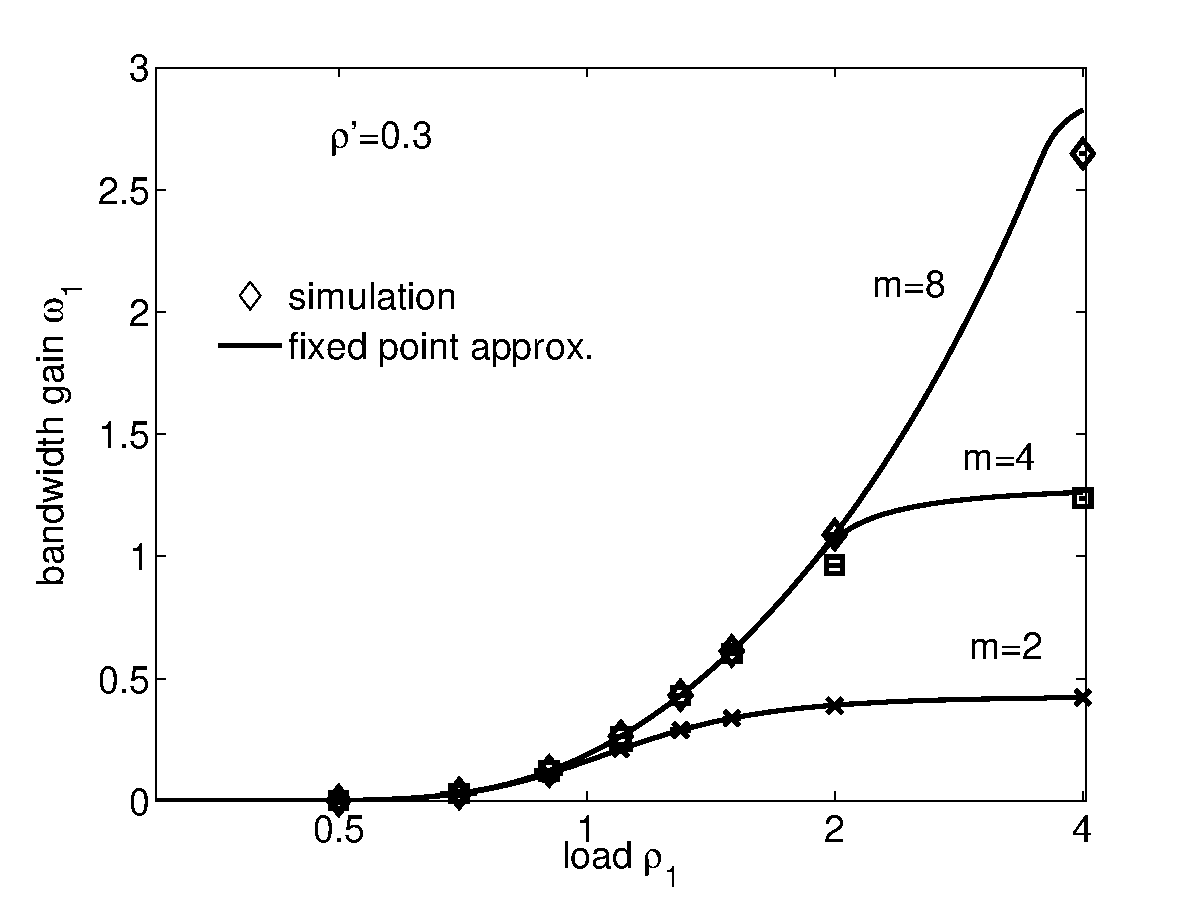
\includegraphics[width=\linewidth]{aggregation/performance_model/figures/fp_bwgain_rho03}
  \caption{Off peak ($\rho'=0.3$)}
  \label{fig:fp_bwgain_rho03}
\end{subfigure}%
\begin{subfigure}{.32\textwidth}
  \centering
  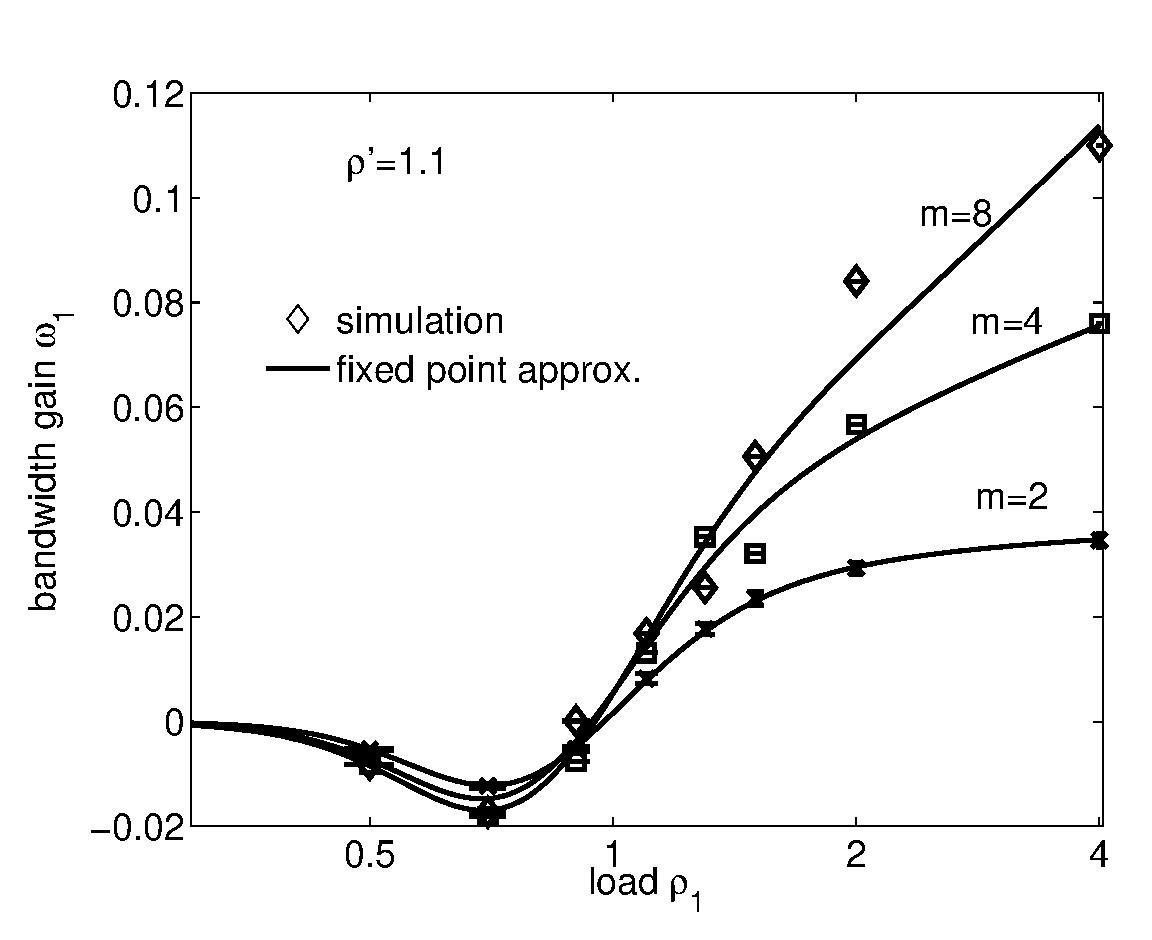
\includegraphics[width=\linewidth]{aggregation/performance_model/figures/fp_bwgain_rho11}
  \caption{Overload ($\rho'=1.1$)}
  \label{fig:fp_bwgain_rho11}
\end{subfigure}
\begin{subfigure}{.32\textwidth}
  \centering
\includegraphics[width=\linewidth]{aggregation/performance_model/figures/fp_bwgain_prio11}
  	\caption{Unfair: ($\alpha_1 \neq \alpha'$)}
  	\label{fig:fp_bwgain_prio11}
\end{subfigure}
\caption{Bandwidth gain dependent on load of the observed system in off peak, overload and unfair operation.}
\label{fig:m82}
\end{figure*}

Figure~\ref{fig:fp_bwgain_rho03} shows the bandwidth gain of the observed system $\omega_1$ dependent on the number of cooperating systems $m$ for $\rho'=0.3$.
Hence, in this case there is a high potential to obtain spare bandwidth from the cooperating systems.
%Independent of the number of cooperating systems $m$, the bandwidth gain increases with the load $\rho_1$ on the observed system.
Depending on the number of cooperating systems the bandwidth gain of the observed system is limited.
%Up to a load of $\rho_1=1$, the spare bandwidth of one underutilized system with $\rho'=0.3$ is enough to support the observed system, which achieves the same bandwidth gain as with more cooperating systems.
%The bandwidth gain is equal for 4 and 8 cooperating systems up to a load of $\rho_1=2$.
%For higher loads of the observed system, the bandwidth that can be provided by 4 cooperating links reaches its limit.
%Especially if the number of cooperating systems is high, an overloaded system gains a lot of bandwidth.

Figure~\ref{fig:fp_bwgain_rho11} shows the bandwidth gain of the observed system $\omega_1$ dependent on the number of cooperating systems $m$ for $\rho'=1.1$.
In this case the links in the composite system are overloaded.
This leads to a loss of up to 2\% bandwidth, if the observed system is not overloaded itself.
If the load on the observed system is high, but low enough that it supports other systems, a traffic burst is more likely to block the system, since the overall load is higher than in the partitioning case.
%If the observed system is also overloaded its bandwidth gain increases dependent on the number of cooperating systems.

To conclude, if the load on the other systems is low, an overloaded system can highly profit from their spare bandwidth by gaining multiples of its own bandwidth. The maximum bandwidth gain is limited by the number of cooperating systems $m$.
If the cooperating systems are overloaded, the received bandwidth might be up to 2\% lower in some cases, but this is compensated with multiples of the base level bandwidth in high peak periods.

%\begin{figure}[tb]
%	\centering
% 	\includegraphics[width=0.5\textwidth]{figures/fp_bwgain_prio11}
%  	\caption{Bandwidth gain dependent on the load of the observed system in egoistic ($\alpha_1$=0\%,$\alpha'$=70\%), normal ($\alpha_1$=70\%,$\alpha'$=70\%) and altruistic ($\alpha_1$=70\%,$\alpha'$=0\%) operation.}
%  	\label{fig:fp_bwgain_prio11}
%\end{figure}

To prevent a system from being congested from an overloaded cooperating system, it can be prioritized. One possibility of prioritizing is to decrease the support threshold $\alpha$, so that it still can offload to other systems, but shares less bandwidth fractions to support. Figure~\ref{fig:fp_bwgain_prio11} shows the bandwidth gain of the observed system for three cases. The dotted line shows the blocking probability if observed and other systems have equal support threshold $\alpha_1=\alpha'=70\%$. The solid line shows the case where the observed system is altruistic and keeps its threshold at $\alpha_1=70\%$, but interacts with egoistic cooperating systems with support threshold $\alpha'=0\%$. The dashed line shows the egoistic case where the observed system limits its support threshold to $\alpha_1=0\%$, while the cooperating systems support up to $\alpha'=70\%$. The altruistic system suffers from egoistic cooperating systems by losing up to about 3\% bandwidth while not being able to gain bandwidth in high loads. Compared to that, the bandwidth gain in the egoistic case is never negative.
Hence, if a system is egoistic it always gains more bandwidth. However, the gain compared to normal operation is not high, and if each system would be egoistic no bandwidth can be shared. This would mean completely partitioned systems which would not change the current situation without bandwidth sharing.
On the other hand, if a system is the only one sharing among only free riders, which corresponds to the altruistic case, the situation is not worse, since only about 3\% of the bandwidth are lost.
Thus it is a win-win situation if everybody contributes to the system and shares spare bandwidth.
This provides incentives for systems to contribute.
%However, losing only up to about 3\% bandwidth in the case, where $m-1=7$ egoistic systems with high load ($\rho'=1.1$) are trying to exploit an altruistic system, shows that the mechanism is quite robust against free riders.
%The gain of the egoistic system decreases with the load of the cooperating system.
%Hence, prioritizing is only viable if the cooperating system is highly loaded.

\subsection{Simulation with General Service Times}\label{sec:simgeneral}

To assess the system performance in more general cases we run simulations with different service time distributions.
Figure~\ref{fig:m2_n20_rho2_sim} shows the blocking probability of the reference system dependent on the load of the systems. The mean values with 95\% confidence intervals of 8 simulation runs are plotted for the service time distributions Deterministic and Hyper-exponential.
The service times in the Deterministic process are constant.
In the Hyper-exponential process we use two branches with probabilities 10\% and 90\%.
For constant service times the blocking probability does not differ from the analytic model for high system loads. The blocking probability differs slightly from the analytic model for Deterministic service times in low system loads, showing higher blocking probabilities if the load on the cooperating system is high. The reason for this has to be investigated and is part of future work. In case of the Hyper-exponential distribution the service times are highly variant. Here the system which is highly loaded benefits from lower blocking probabilities compared to the analytic model.

\begin{figure}[tb]
	\centering
	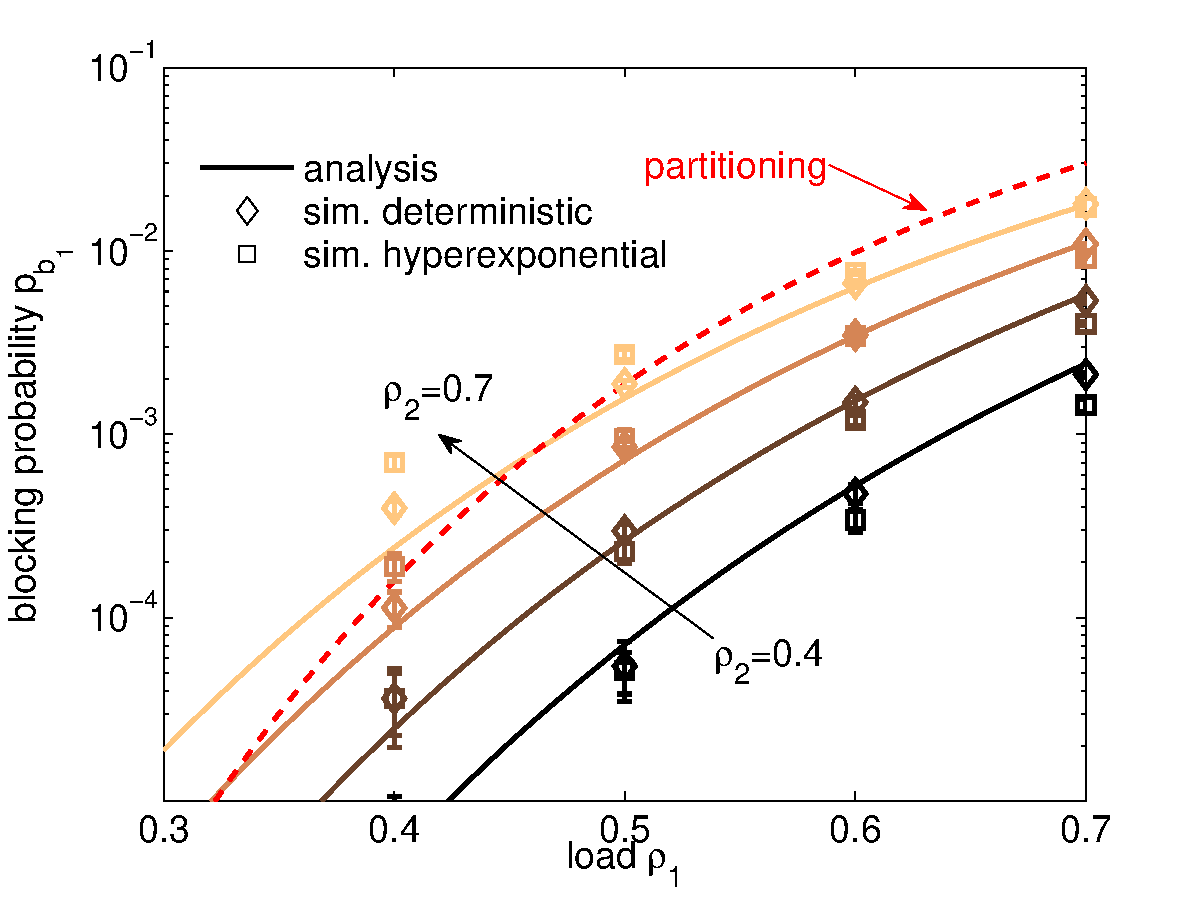
\includegraphics[width=0.5\textwidth]{aggregation/performance_model/figures/m2_n20_rho2_sim}
 	\caption{Blocking probability dependent on the load of reference and cooperating system. Simulation with different service time distributions.}
 	\label{fig:m2_n20_rho2_sim}
\end{figure}

In Figure~\ref{fig:bw_n20_rho2_sim}, which shows the available bandwidth of the reference system dependent on the load, simulation results are plotted for Deterministic distributed and highly variant Hyper-exponential distributed service times.
For Deterministic service times the analytic model fits the simulation results. If the service times are highly variant the reference system receives only slightly more bandwidth than in the model if it is overloaded. Hence, considering the available bandwidth the analytic model can be used to assess the system performance with general service time distributions.

% \begin{figure}[tb]
% 	\centering
% 	\includegraphics[width=0.5\textwidth]{aggregation/performance_model/figures/m2_n20_q1}
%  	\caption{Blocking probability of two queues dependent on load.}
%  	\label{fig:m2_rho2_q1}
% \end{figure}


\section{Lessons Learned}\label{sec:aslevel:lessons_learned}
In this chapter we characterize content delivery networks on AS level. %by evaluating measurements of the most common content delivery principles P2P and CDN.
For that purpose we summarize related work and use measurements conducted on the distributed platform PlanetLab and a crowdsourcing platform.
To assess the potential of content delivery approaches that use local resources, we determine the number of active IP-addresses from the Internet Census dataset.

%P2P -> CDN
%to accurately model content delivery networks ... is described.
%While ... we find three major outcomes.
First, we provide a comprehensive overview on content delivery network concepts and their evolution. We briefly describe the structure of the YouTube CDN and describe the concept of the next generation of hierarchical CDNs, which use local resources to support content delivery.
In order assess the number of local resources available in each AS, we analyze the Internet Census Dataset to derive the distribution of IP-addresses on ASs.
To this end, we use a mapping of IP-addresses to AS numbers.
we find that the distribution of IP-addresses is highly heterogeneous showing that 30\% of the active IPs belong to the 10 largest ASs.
This means that the potential of approaches that use resources on home routers highly depend on the ISP network.

Second, we propose the usage of crowdsourcing platforms for distributed network measurements to increase the coverage of vantage points.
We evaluate the capability to discover global networks by comparing the coverage of video server detected, using a crowdsourcing platform as opposed to using the PlanetLab platform.
To this end, we use exemplary measurements of the global video CDN YouTube, conducted in both the PlanetLab platform as well as the crowdsourcing platform Microworkers.
Our results show that the vantage points of the concurring measurement platforms have very different characteristics.
We show that the distribution of vantage points has high impact on the capability of measuring a global content distribution network.
The capability of PlanetLab to measure a global CDNs is rather low, since 80\% of requests are directed to the United States.
Our results confirm that the coverage of vantage points is increased by crowdsourcing.
Using the crowdsourcing platform we obtain a diverse set of vantage points that reveals more than twice as many autonomous systems deploying video servers than the widely used PlanetLab platform.
%Part of future work is to determine if the coverage of vantage points can be even further increased by targeting workers from specific locations to get representative measurement points for all parts of the world.

Finally, we investigate where in the Internet BitTorrent traffic is located and which ISPs benefit from its optimization. We use measurements of live BitTorrent swarms to derive the location of BitTorrent peers and data provided by Caida.org to calculate the actual AS path between any two peers.
Our results show that the traffic optimization potential depends heavily on the type of ISP.
Different ISPs will pursue different strategies to increase revenues.
Our results confirm that selecting peers based on their locality has a high potential to shorten AS paths between peers and to optimize the overlay network. In the observed BitTorrent swarms twice as much traffic can be kept intra-AS using locality peer selection. Thus, the inter-AS traffic is almost reduced by \unit[50]{\%} in \tier and in large ISPs.
%If ...
%This would for example allow ..

Based on the results obtained in this chapter, we develop models that describe the characteristics of CDNs and the number of active subscribers in ISP networks.
The models allow us to analyze the performance of traffic management mechanisms in realistic scenarios.
%Upper bounds / potential of p2p cdn approach.
%Including the application providers as stakeholders and considering their key performance indicators requires new models but also allows us to better understand the impact of mechanisms implemented in applications.
%Key performance indicators of application providers sometimes overlap with those relevant to users, as application providers try to improve the experience of users in order to reduce churn.

%Highlighted by both, the P2P approach and the CDN approach the distribution of peers on autonomous systems and the popularity of content is highly heterogeneous.
%Dynamics (orange paper)
%While general traffic management mechanisms intent to optimize the cdn
%this only increases the efficiency of the ISP cache, which may cause suboptimal results if the popularity of videos large variance.
%Thus, we suggest to  tradeoffs, within reason, to the user.
%This approach could be seen as extending the \emph{Economic Traffic Management} approach to the user.

